\documentclass{beamer}
\usepackage{amsmath,amssymb,amsfonts,mathrsfs,accents}
\usepackage{array}
\usepackage{graphicx}
\usepackage{caption}
\usepackage{subcaption}
\usepackage[utf8]{inputenc}
%\usetheme{Madrid}
\usecolortheme{default}
\usepackage{blindtext}
\usepackage{hyperref}
\usepackage{multirow}
\usepackage{appendixnumberbeamer}
\setbeamertemplate{caption}[numbered]
\setbeamertemplate{page number in head/foot}[appendixframenumber]
\usepackage{listings}
\usepackage[authoryear]{natbib}
\bibliographystyle{plainnat} 
\renewcommand{\lstlistingname}{Model}
\lstset{frame=none, framexleftmargin=4pt, framexrightmargin=4pt, backgroundcolor=\color{code_bg}, basicstyle=\footnotesize\ttfamily, tabsize=2}

%For different theme%%%%%%%%%%%%%%%%%
\usetheme[progressbar=frametitle]{metropolis}
\usepackage{appendixnumberbeamer}

\usepackage{booktabs}
\usepackage[scale=2]{ccicons}

\usepackage{pgfplots}
\usepgfplotslibrary{dateplot}

\usepackage{xspace}
\newcommand{\themename}{\textbf{\textsc{metropolis}}\xspace}
%%%%%%%%%%%%%%%%%%%%%%%%%%%%%%%%


% Custom footline with increased height

% \setbeamertemplate{footline}{
%     \leavevmode%
%     \hbox{%
%         \begin{beamercolorbox}[wd=\paperwidth,ht=3.5ex,dp=1.5ex,center]{author in head/foot}%
%             \usebeamerfont{author in head/foot}\insertshortauthor \hspace*{2em} \insertshorttitle \hspace*{2em} \insertshortdate{} \hspace*{2em} \insertframenumber/\inserttotalframenumber
%         \end{beamercolorbox}%
%     }%
%     \vskip0pt%
% }

% % Custom color definition for a lighter blue shade
% \definecolor{lighterblue}{RGB}{50, 50, 150}  % Adjust the RGB values for the lighter blue

% Change headline (frame title bar) height and color
%\setbeamertemplate{frametitle}{
%    \nointerlineskip
%    \vbox{
%        \begin{beamercolorbox}[wd=\paperwidth,ht=3ex,dp=2ex,center]{frametitle} % Adjust height here
%            \usebeamerfont{frametitle}\insertframetitle
%        \end{beamercolorbox}
%    }
%}

% Set headline (frame title) background color to the custom lighter blue
%\setbeamercolor{frametitle}{bg=lighterblue,fg=white}

% Customize the title page color (title box) with the same color as the headline
%\setbeamercolor{title}{bg=lighterblue,fg=white}
%\setbeamercolor{title in headline}{bg=lighterblue,fg=white}


%-----------------------------------------------------------------------------------%

\begin{document}
\title{Power sector transition dynamics}
\author{Maija Kaartinen and Alireza Azampour}
\date{\today}
\maketitle

%----------------------------------------------------------------------------------

\begin{frame}{Power sector transition dynamics}

\begin{itemize}
\item Firms' technology adoption decisions determine the pace of the green transition
\item Their initial technological capital likely plays a role in this
\item Need to analyze the impacts of climate policy through the lens of firm investment choices
 \hfill \break
 \item Climate policies impact firms' investment choices via
 \begin{itemize}
     \item Operation costs: carbon taxes
     \item Fixed costs: installation subsidies
     \item Demand side: feed-in tariffs and renewable energy mandates
 \end{itemize}
 \item How do these impact the pace of transition?

\end{itemize}
\end{frame}
%%%%%%%%%%%%%%%
\begin{frame}{US power sector: two transitions}\label{transition0}


\begin{table}
\centering
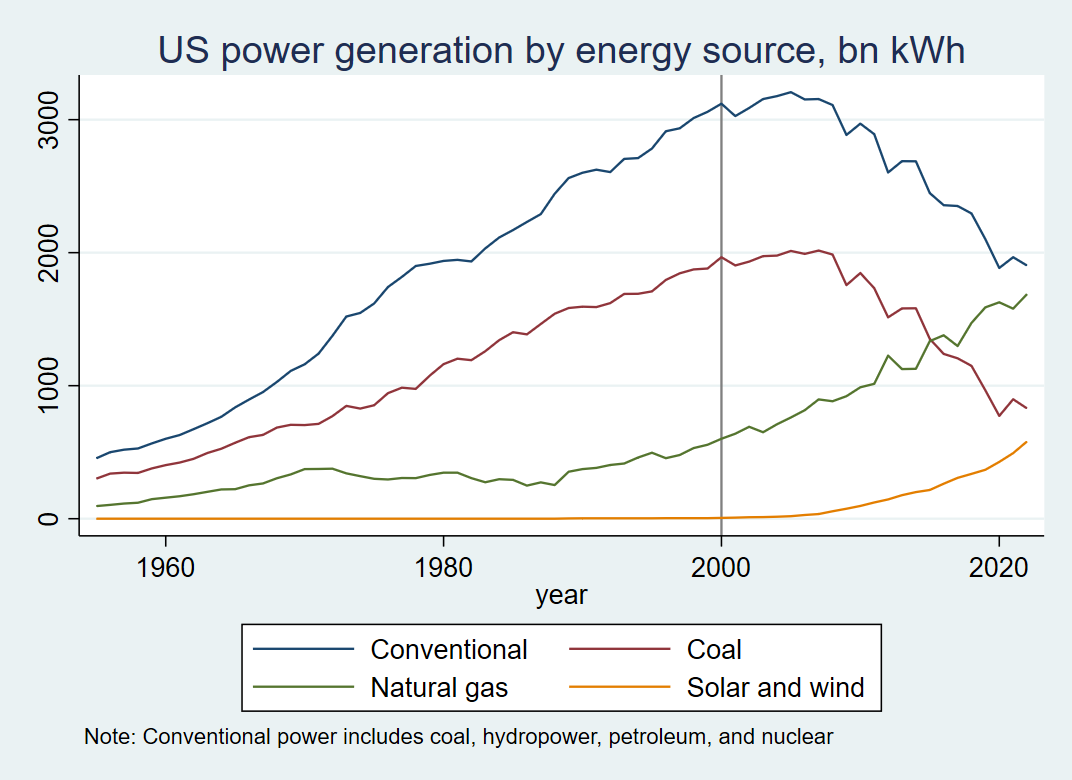
\includegraphics[scale=0.25]{US_powergeneration_trends.png}
\end{table}

\hyperlink{transit_measure}{\beamerbutton{Model results}}
\end{frame}
    
%%%%%%%%%%%%%%%
\begin{frame}{Transition 1: Conventional fuels to natural gas}\label{gasindata}

\begin{center}
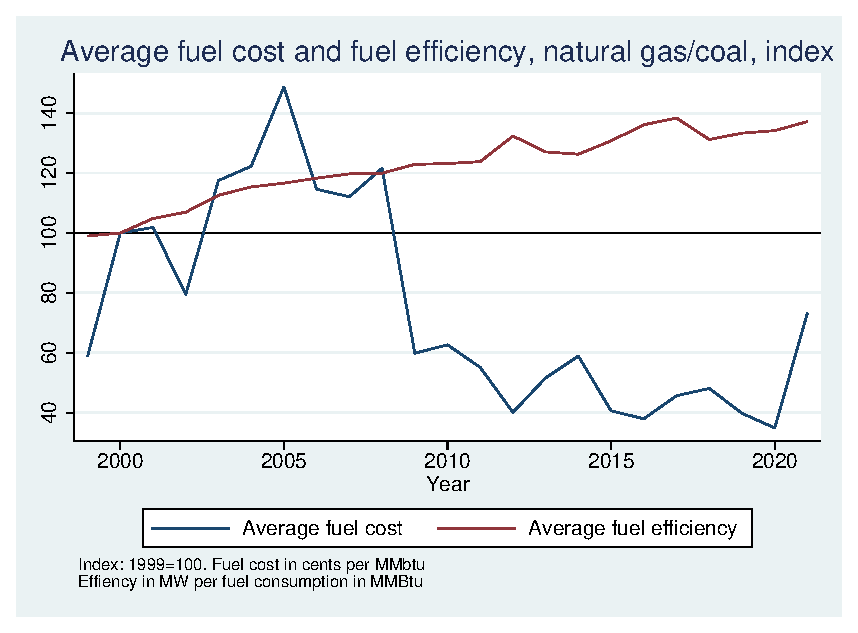
\includegraphics[scale=0.65]{NG_cost_effic_coalcomp.eps}
\end{center}
\hyperlink{transit_shocks1}{\beamerbutton{Shocks in model}} \hyperlink{transit_NGprice}{\beamerbutton{Price in model}}
\end{frame}
%%%%%%%%%%%%%%%

\begin{frame}{Transition 2: Conventional fuels to solar and wind}

\begin{figure}
\centering
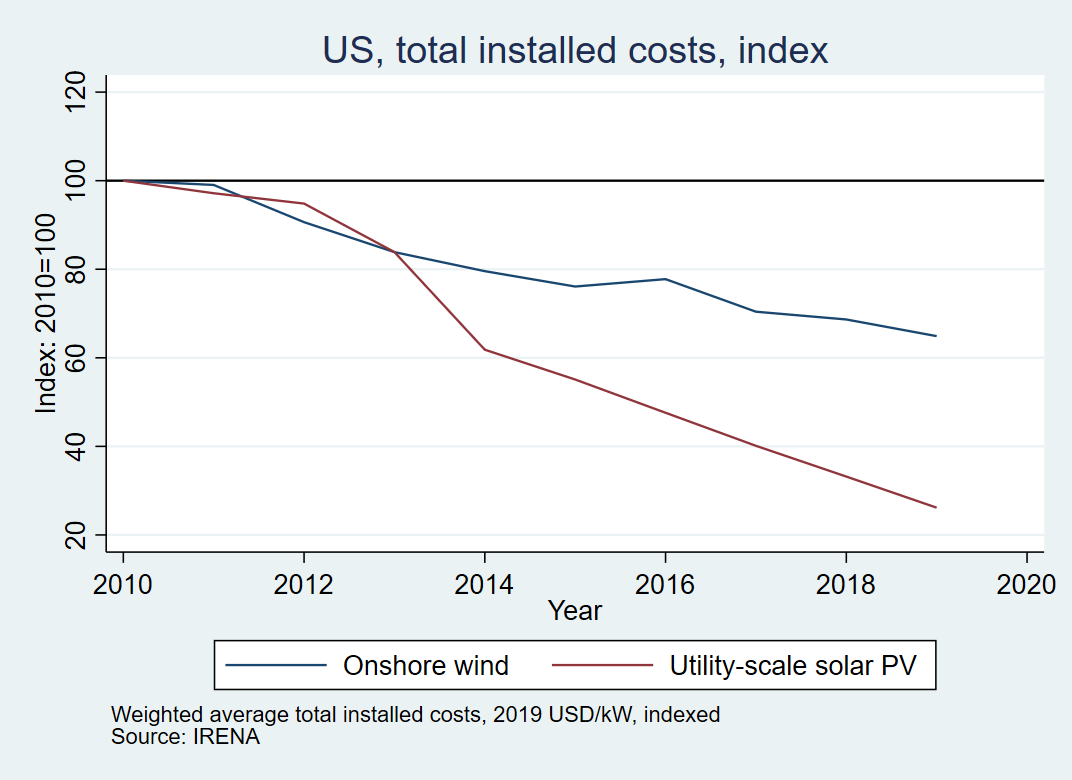
\includegraphics[scale=0.25]{solarwind_installedcosts_index.png}
\end{figure}

    
\end{frame}
%%%%%%%%%%%%%%%

\begin{frame}{Research question}
\large 
\begin{center}
    \textbf{"What determines the pace of technological transition in the power sector?"}\\\\
\hfill \break
\hfill \break
\begin{itemize}
    \item Primary goal: analyze the effects of power sector climate policies 
    \item In addition, a micro-founded alternative for canon CES models
\end{itemize}
\end{center}
\end{frame}

%%%%%%%%%%%%%%%

\begin{frame}{Outline of the project}

\begin{itemize}
    \item We present a heterogeneous agent power sector model, with generator-level technology adoption decisions.
    \item Data on US power generators is used to test its implications
    \item The model is calibrated to match the transitions towards
    \begin{enumerate}
        \item Natural gas
        \item Solar and wind
    \end{enumerate}
    \item Counterfactual analysis to test the implications of power sector policies.
\end{itemize}

    
\end{frame}
%%%%%%%%%%%%%%%
\begin{frame}{Previous literature}
\small
\begin{itemize}
        \item Green transition and energy policy:\\\\ \cite{NBERw31615}, \cite{gentile}, \cite{shapiro2018pollution}, \cite{10.1257/aer.102.1.131}, \cite{NBERw18456}, \cite{NBERw31657}
        \item IO literature on the energy sector:\\\\ \cite{cff33ae3-b2ce-366e-bebc-18cca840e11c}, \cite{10.1257/aer.20172034}, \cite{Mackay}
        \item Technology adoption and productivity: \\ \cite{b541c6d5-0739-3bb5-b854-210c9c94396d}, \cite{benhabib}
        \item Firm turnover and structural change:\\\\ \cite{hopenhayn}, \cite{luttmer_selection_2007}
\end{itemize}

    
\end{frame}
%%%%%%%%%%%%%%%
\begin{frame}{Patterns in the data: technology adoption}\label{Facts}

\begin{enumerate}
\item A generator's efficiency relative to the market declines over time, in the absence of technological updates.
\item A generator's efficiency is persistent across periods and technology updates.
\item The more time that has passed since the previous update, the higher the likelihood of an update.
\item The higher the efficiency after the previous update, the lower the likelihood of an update.
\item Generators with higher persistent quality depreciate slower.

\end{enumerate}

\hyperlink{Data}{\beamerbutton{Data }}
    
\end{frame}
%%%%%%%%%%%%%%%

\begin{frame}{The model}\label{model_struct}
\small
\begin{itemize}
 \item Generators produce in a competitive market using a fuel input.
 \item They belong to one of two technology types: old or new.
 \item The productivity of each generator depends on the effective age and efficiency of their technology.
 \item In each period, a generator can choose to pay an adoption cost and update to a new efficiency value. The value is stochastic but known before paying the cost. 
 \item A generator exits if its present value goes to zero.
 \item Entrants can pay an entry cost and draw an initial efficiency value $a_{i,0}$ in either technology.
 \item Entry and exit is the main margin for transition from the old to new technology.
\end{itemize}

    \hyperlink{definitions}{\beamerbutton{Definitions}}  
\end{frame}
%%%%%%%%%%%%%%%
\begin{frame}{The model: market structure}
\small
\begin{itemize}
 \item Generators use the fuel input $e_i^o$ or $e_i^n$ at prices $p^o$ or $p^n$, respectively
  \item Both types sell electricity at the price $p_E$
 \item Productivities are drawn from a normal distribution with mean $\overline{a}^o$ or $\overline{a}^n$ with the same variance $\sigma$: productivity growth is exogenous
 \item The two types pay technology adoption costs $c_a^o$ and $c_a^n$ and operation costs $c_f^o$ and $c_f^n$
 \hfill \break
 \item Electricity demand is given by: $\ln(d_E) = \ln d_0-\varepsilon_E\ln(p_E)$
 \item The supply of fuel input j is given by:  $\ln e_s^j = \ln e_s^{0,j}+\epsilon_s \ln p^j$

\end{itemize}
    
\end{frame}
%%%%%%%%%%%%%%%
\begin{frame}{The model: generator's period problem}\label{gen_problem}
\begin{itemize}
\item The generator's period profits are given by:
\begin{equation*}
    p_E\frac{a_{i}^{1+\gamma t}}{(1+g_a)^t} e_i^\alpha -p_e e_i-c_f
\end{equation*}

\item Where $\alpha<1$ and $\gamma>0$
 \item The term: \begin{equation*}
     \frac{a_{i}^{1+\gamma t}}{(1+g_a)^t}
 \end{equation*} is the generator's efficiency relative to the market
 \item $g_a$ is the rate at which a generator's relative efficiency declines
    
\end{itemize}

 \hyperlink{intra_period}{\beamerbutton{Intra-period problem}}  
 \hyperlink{alt_model}{\beamerbutton{Alternative model}}   
  \hyperlink{effic_between_model}{\beamerbutton{Calibration}}
  \hyperlink{coal_gas}{\beamerbutton{Coal-gas switching}}  

    
\end{frame}
%%%%%%%%%%%%%%%
\begin{frame}{The model: generator value function}\label{value_fn}
\begin{itemize}
\item The value function is given by:
\begin{align*} 
    v(a_{i},t) &= \max_{e_i,ad=\{0,1\}} p_E\frac{a_{i}^{1+\gamma t}}{(1+g_a)^t} e_i^\alpha -p_e e_i-c_f\\ 
    &+\beta \big(\mathbf{1}_{\{ad =0\}} \mathbb{E}[v(a_{i},t+1)]  + \mathbf{1}_{\{ad =1\}}[ \mathbb{E}[v(a_{i}',t-\tau)]-c_a]\big)
\end{align*}
\hfill\break
    \item Technology draws follow $a'_i\sim \rho a_i + (1-\rho)\epsilon_i$ where $\epsilon_i$ follows an $i.i.d$ normal distribution with the same parameters as of the entrants' distribution
     \item $\tau$ is the reduction in technological age following an update
    
\end{itemize}

 \hyperlink{intra_period}{\beamerbutton{Intra-period problem}}  
 \hyperlink{alt_model}{\beamerbutton{Alternative model}}   
  \hyperlink{effic_between_model}{\beamerbutton{Calibration}}
\hyperlink{coal_gas}{\beamerbutton{Coal-gas switching}}    
    
\end{frame}
%%%%%%%%%%%%%%%
\begin{frame}{The model: entry and exit}
\begin{itemize}
    \item The value of entry is given by: 
    \begin{equation*}
    \begin{aligned} 
    E[v(a_{i,0},0)]-c_{e}&=\\\int \big\{ p_Ea_{i,0} e_i^\alpha &-p_e e_i+E[v(a_{i,0},1)] \big\} dD(a_{i,0})-c_{e}
\end{aligned}
    \end{equation*}
    
where $c_{e}$ is the entry cost and $a_{i,0}$ is drawn from the exponential distribution
\hfill \break
    \item If $v<0$ the generator exits
\end{itemize}
    
\end{frame}
%%%%%%%%%%%%%%%
\begin{frame}{Equilibrium}
The Equilibrium consists of policy function $P(a_i,t)$, a stationary distribution of generators $\Gamma$ with the measure $m_{ss}$, and an equilibrium price $p_E$ where:
    \begin{itemize}
        \item  $P(a_i,t)$ is the answer to firms' problem at the price $p_E$
        \item The electricity market clears at the price $p_E$ 
        \item The fuel input markets clear at prices $p_e^o$ and $p_e^n$
        \item The value of entry is zero, or the the mass of generators is zero for both technology types
    \end{itemize}
     \hyperlink{alt_model}{\beamerbutton{Alternative model}} 
\end{frame}



%%%%%%%%%%%%%%%%%%%%%%%%%%%%%%%%%%%%%%%%%%%%%%%%%%%%%%%%%%%%%%%%%%%

\begin{frame}{Data: EIA power generator data}\label{Data}

\begin{itemize}
 \item EIA US power generator data from years 1991-2021.
 \item Utility power plants until year 2000: all power plants included thereafter. 
 \item Unbalanced panel.
 \item Generator-level data on capacity, energy sources, operating status, planned modifications, first year of operation, location, owner, and power plant.
 \item Plant-level data on net generation and fuel consumption.
  \item The data analysis only covers operating generators that use a fuel.


\end{itemize}

\hyperlink{Facts}{\beamerbutton{Data patterns}}
\end{frame}
%%%%%%%%%%%%%%%
\begin{frame}{Variables constructed for analysis}\label{variables}

 \begin{itemize}
     \item Efficiency: fuel consumption per unit of net generation.
     \item Efficiency update dummy: 1 when efficiency increases by 5\% or more but the ratio between capacity and generation does not change by more than 10\% (we test several thresholds).
     \item Technological age variable: number of years since the latest update.
     \item Plant's persistent quality: average technological age at the time of update.
 \end{itemize}
 
\hyperlink{efficall_dist}{\beamerbutton{Efficiency}}
\hyperlink{Years since latest update}{\beamerbutton{Technological age}}
    
\end{frame}

%%%%%%%%%%%%%%%

\begin{frame}{Data: Technology adoption patterns}\label{patterns_1gen}
\begin{table}
\footnotesize
\centering
\caption{Update dummy regressed on covariates, single-generator plants}
\scriptsize
\begin{tabular}{lcc} \hline
 & (1) & (2) \\
VARIABLES & Raw data & Fixed effects \\ \hline
 &  &  \\
Relative efficiency after latest upgrade & -0.0630*** & -0.248*** \\
 & (0.0123) & (0.0916) \\
Years since latest update & -0.00432*** & 0.00738*** \\
 & (0.000760) & (0.00164) \\
Constant & 0.156*** & 0.308*** \\
 & (0.0149) & (0.0933) \\
 &  &  \\
Observations & 3,356 & 3,242 \\
 Adjusted R-squared & 0.014 & 0.054 \\ \hline
\multicolumn{3}{c}{ Robust standard errors in parentheses} \\
\multicolumn{3}{c}{ *** p$<$0.01, ** p$<$0.05, * p$<$0.1} \\
\end{tabular}

\end{table}
\tiny{Note: Update dummy defined as efficiency increase of at least 5\% with less than 10\% change in the capacity-to-generation ratio }

\hyperlink{patterns_all}{\beamerbutton{All plants}}
\hyperlink{obscount}{\beamerbutton{No of observations}}
\hyperlink{updatespattern}{\beamerbutton{Histogram}}
\end{frame}

%%%%%%%%%%%%%

\begin{frame}{Calibration, first steady state in coal to gas transition}\label{calibration}
\tiny
\begin{tabular}{ |p{1.1cm}p{3.5cm}p{1.4cm}p{3.2cm}|  }
 \hline
 \multicolumn{4}{|c|}{Externally calibrated} \\
 \hline
 \textbf{Param.} & \textbf{Description} & \textbf{Value} & \textbf{Source}\\
 $c_{o,e}/c_{n,e}$   & Construction cost    & 2.8 &   Overhead cost, EIA \footnotemark[1]\\
 $c_{o,f}/c_{n,f}$ &   Fixed operating cost  & 2   & Fixed O\&M cost, EIA \footnotemark[1] \\
$f(\epsilon_{o,i})$ & Draw distribution, coal & $\mathcal{N}(0.3, 0.12)$ & New plant efficiency values\footnotemark[2] \\
$ f(\epsilon_{n,i})$ & Draw distribution, gas & $\mathcal{N}(0.4, 0.12)$ & New plant efficiency values\footnotemark[2] \\
 $\rho$ &   Draw autocorrelation  & 0.7 & Plant efficiency values\\
  $\gamma$ &   Quality persistence  & 0.0075 & Depreciation estimates \footnotemark[2]\\
 $g_t$ &   Obsolescence rate  & 0.015 & Depreciation estimates \footnotemark[2]\\
 \epsilon_i &  Coal/gas supply elasticity &  0.4  & Arora and Vipin, 2014 \footnotemark[3] \\
    \varepsilon_E    &  Electricity demand elasticity &  1  & Burke and Abayasekara, 2018 \footnotemark[3]\\
 $\beta$   & Depreciation rate   & 0.97 &   \\
 \hline
  \multicolumn{4}{|c|}{Internally calibrated} \\
  \hline
  \textbf{Param.} & \textbf{Description} & \textbf{Value} & \textbf{Matching Moment} \\
  $\alpha$   & Prod. function curvature    & 0.7125 &  Input use ratio $\overline{e}_o/\overline{e}_n$ \\
 $\frac{c_{o,a}}{c_{n,a}}, \frac{c_{o,a}}{c_{o,e}} $ &   Adoption cost ratio & 1,\ 9.6\%  &  Mean effic. and capacity ratio \\
$e_{s,0}^{o},\:e_{s,0}^{n}$ & Baseline coal/gas supply  & 2.166,\ 0.246  & Input prices \\
 $d_0$ &   Baseline electricity demand  & 9.24 & Electricity price \\
  Exit rate & Plant exit rate  & 1\%   & Plant retirement rate\\
  $\tau$   & Technological age reduction   &  &  mean of years since update  \\
 \hline
\end{tabular}
\footnotetext[1]{\tiny USD/kW, 1997-1999 average from annual "Assumptions to the Annual Energy Outlook"}
\footnotetext[2]{\tiny We back out $\gamma$ from a regression of efficiency values in periods between updates on covariates: \hyperlink{effic_between_model}{\beamerbutton{Estimation}}}
\footnotetext[3]{\tiny Long-run elasticity estimates}
% \footnotetext[4]{\tiny We used age cutoffs to see when the efficiency gain after update started to decrease.}
\end{frame}
%%%%%%%%%%%%%%%
\begin{frame}{Calibration: efficiency distribution, old technology}

\begin{figure}
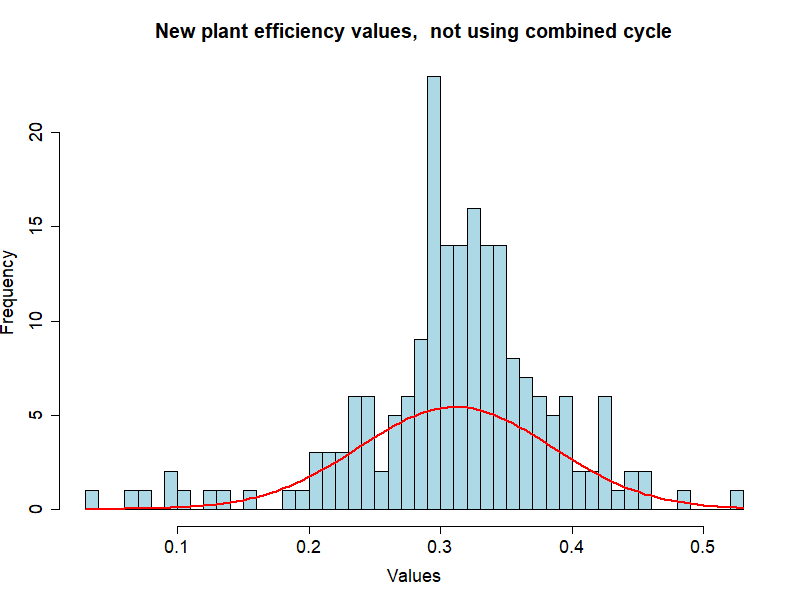
\includegraphics[scale=0.32]{efficdist_noCC_norm_hist.png}
\end{figure}

\hyperlink{updatespattern}{\beamerbutton{Update patterns}}


\end{frame}

%%%%%%%%%%%%%%%

\begin{frame}{Calibration: efficiency distribution, new technology}

\begin{figure}
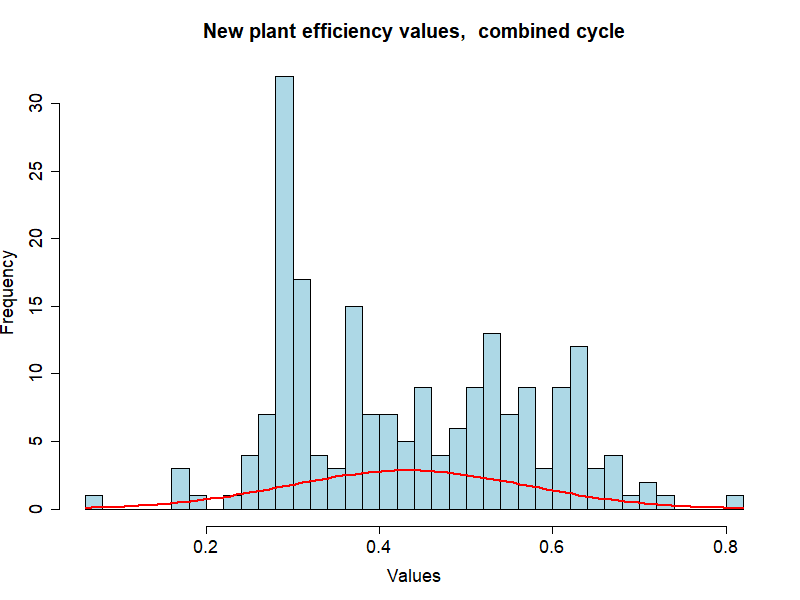
\includegraphics[scale=0.32]{efficdist_CC_norm_hist.png}
\end{figure}

\hyperlink{updatespattern}{\beamerbutton{Update patterns}}

\end{frame}

%%%%%%%%%%%%%%%
\begin{frame}{Calibration: Construction and fixed operating costs}
\begin{figure}
\caption{Overhead and fixed operating costs}
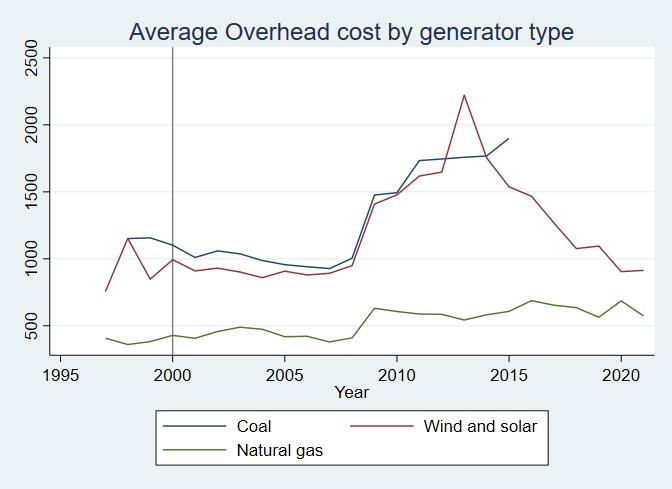
\includegraphics[width=0.53\textwidth]{Overhead cost_trends_gentype_fewer.png}%
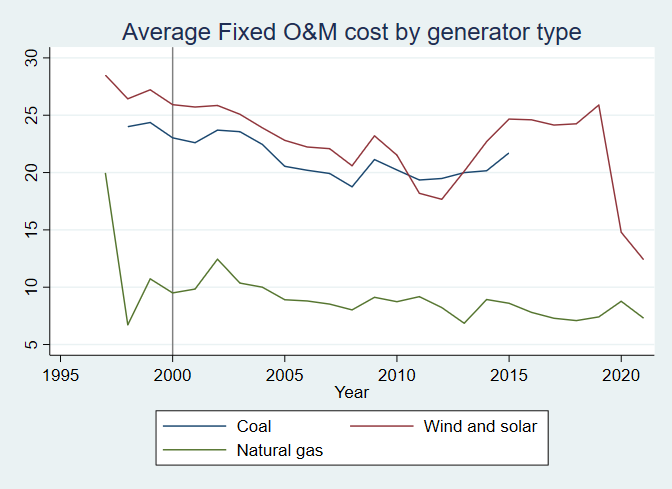
\includegraphics[width=0.53\textwidth]{Fixed O&M cost_trends_gentype_fewer.png}
\end{figure}


\end{frame}

%%%%%%%%%%%%%%%

\begin{frame}{Moments, first steady state in coal to gas transition}
\footnotesize
\begin{tabular}{ |p{1.2cm}|p{2.2cm}|p{4.3cm}|p{0.6cm}|p{0.9cm}|  }
 \hline
   \multicolumn{5}{|c|}{Moments, first steady state} \\
   \hline
  \textbf{Param.} & \textbf{Description} & \textbf{Source} & \textbf{Data} & \textbf{Model} \\
  $cap_o/cap_n$   &  Measure ratio   &  Installed capital ratio, coal/gas & 3.03 & 5.4 \\
 $\overline{a}$ &   Mean efficiency   &  Plant efficiency values, coal/gas & 0.33  &0.39\\
 $\overline{e}_o/\overline{e}_n$ & Input use ratio  & Coal and gas plant fuel cons. & 7.27 & 8.27  \\
  $p^o $ & Input price, old  & Coal price \footnotemark[1] & 1.45& 1.82  \\
  $p^n $ & Input price, new  & Natural gas price \footnotemark[1] & 2.32&2.14\\
  $p_E$ & Electricity price  &  Retail price, industrial clients \footnotemark[1] & 14.06 & 14.97  \\
 \hline
\end{tabular}

\footnotetext[1]{\tiny USD/MMBtu}
\end{frame}
%%%%%%%%%%%%%%%
\begin{frame}{Steady state results}
\begin{figure}
\centering
\caption{Coal power plants: (relative) efficiency distribution before transition}
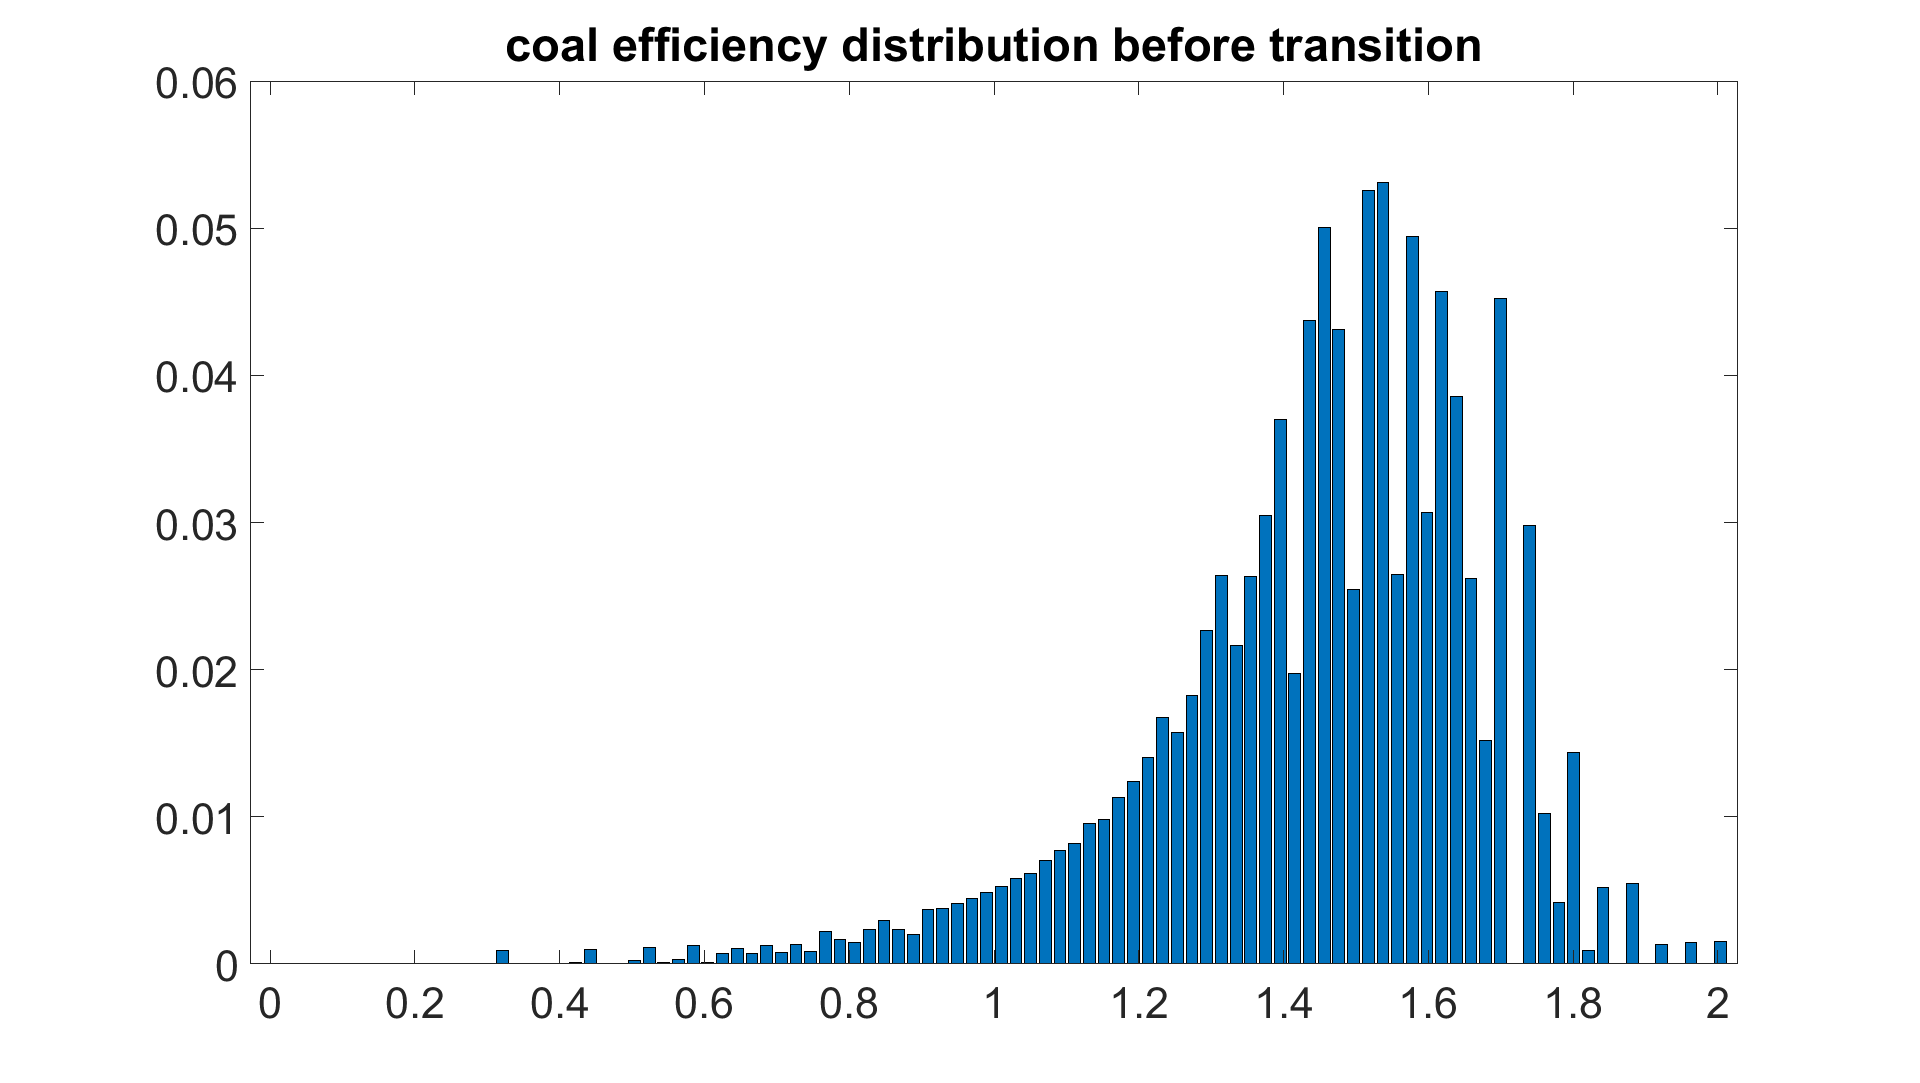
\includegraphics[scale=0.20]{coal efficiency distribution before transition.png}
\end{figure}

\end{frame}

%%%%%%%%%%%%%%%
\begin{frame}{Efficiency distribution, data}\label{efficall_dist}

\begin{figure}
\centering
\caption{Relative efficiency values of all plants, normalized}
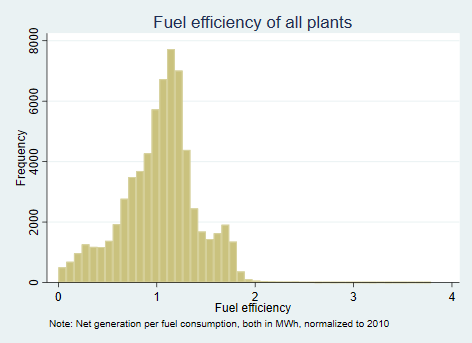
\includegraphics[scale=0.45]{EFFIC_effic_plant_norm_all_hist.png}
\end{figure}
\scriptsize{Note: Technological update implies an efficiency increase of at least 10 \%, with less than 5 \% variation in generator capacity-to-generation ratio}

\hyperlink{efficnew_dist}{\beamerbutton{Efficiency values after update}}
\hyperlink{variables}{\beamerbutton{Variables}}

\end{frame}

%%%%%%%%%%%%%%%%
\begin{frame}{Transition 1: Coal to natural gas}\label{transit_shocks1}
\begin{itemize}
\footnotesize
\item Baseline electricity demand is growing at 1.3\% per year
\item Adjustment cost applied to electricity and input price changes
\item Coal-to-gas transition cost equal to 40\% of natural gas entry cost (EIA)
\end{itemize}

\begin{figure}
\centering
\caption{The path of shocks in the model}
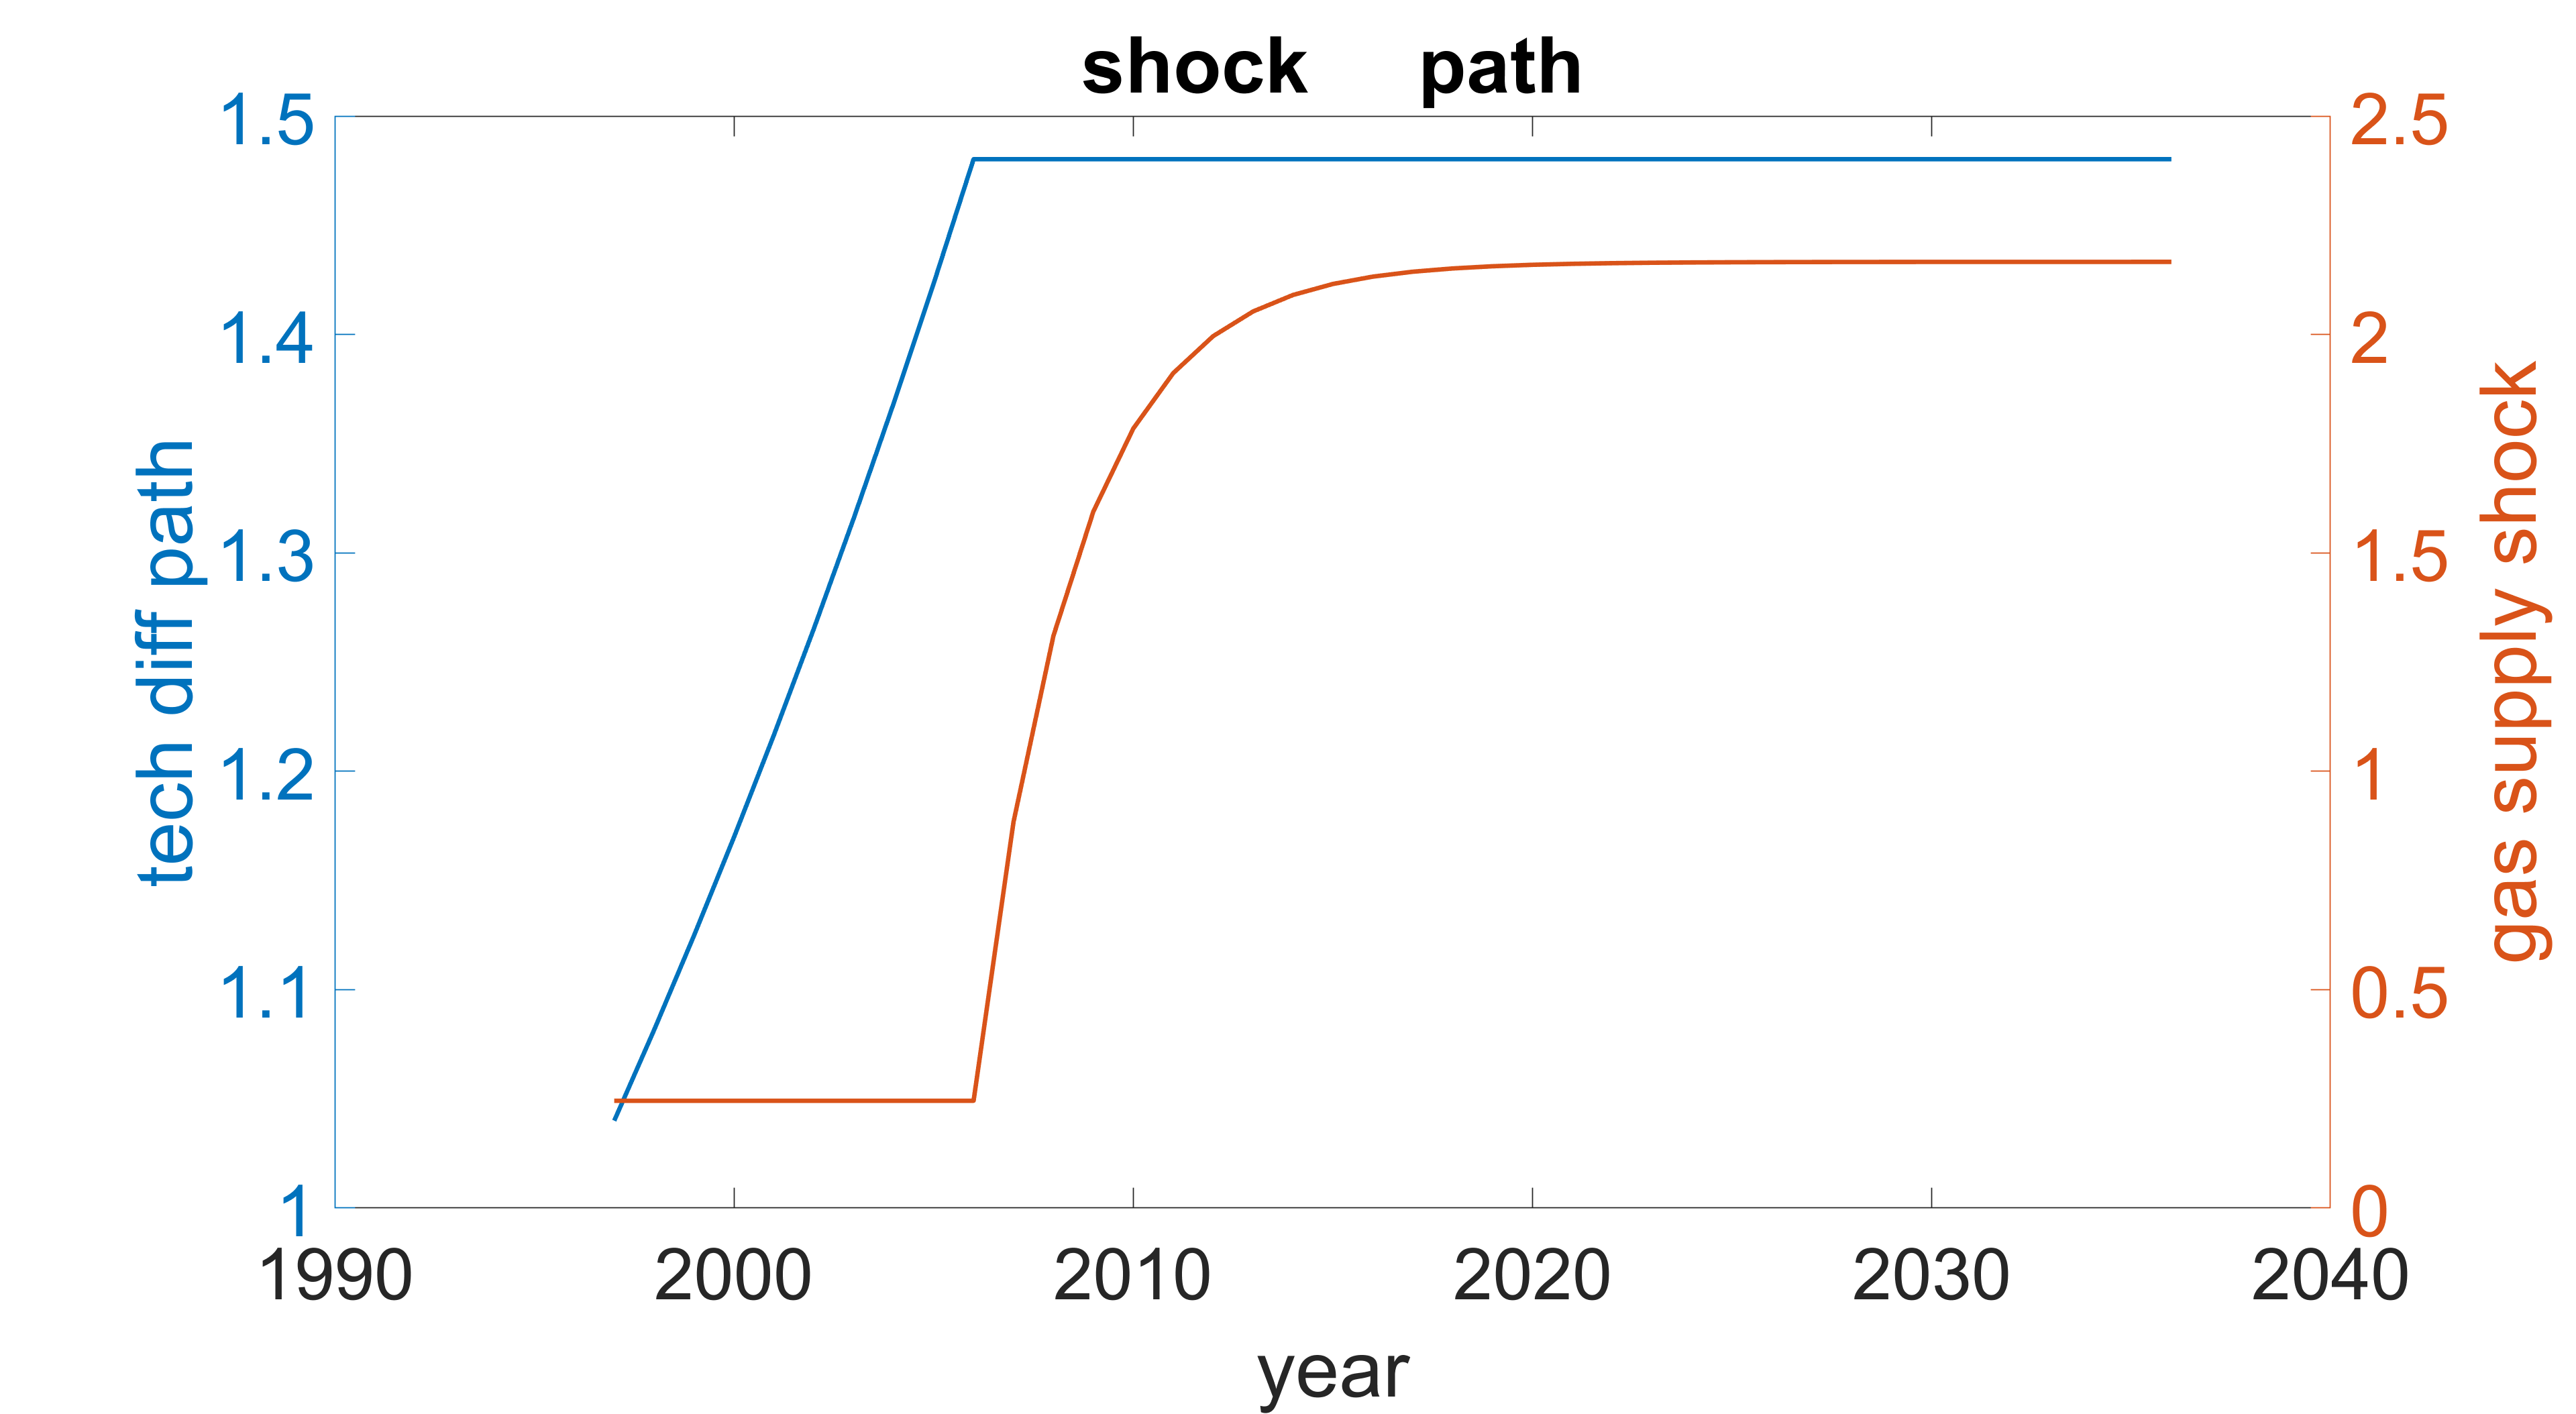
\includegraphics[scale=0.08]{shock path cg2.png}
\end{figure}

\hyperlink{gasindata}{\beamerbutton{Natural gas/coal efficiency and costs}}
\end{frame}
%%%%%%%%%%%%%%%

%%%%%%%%%%%%%%%%
%\begin{frame}{Transition 1: Conventional fuels to natural gas}


%\end{frame}
%%%%%%%%%%%%%%%

%%%%%%%%%%%%%%%%%%%%%%%%%%%%%%%%%%%%%%%%%%%%%%%%%%%%%%%


\begin{frame}{Transition 1: Coal to natural gas}\label{transit_measure}

\begin{figure}
\centering
\caption{Share of gas generation over the convergence path}
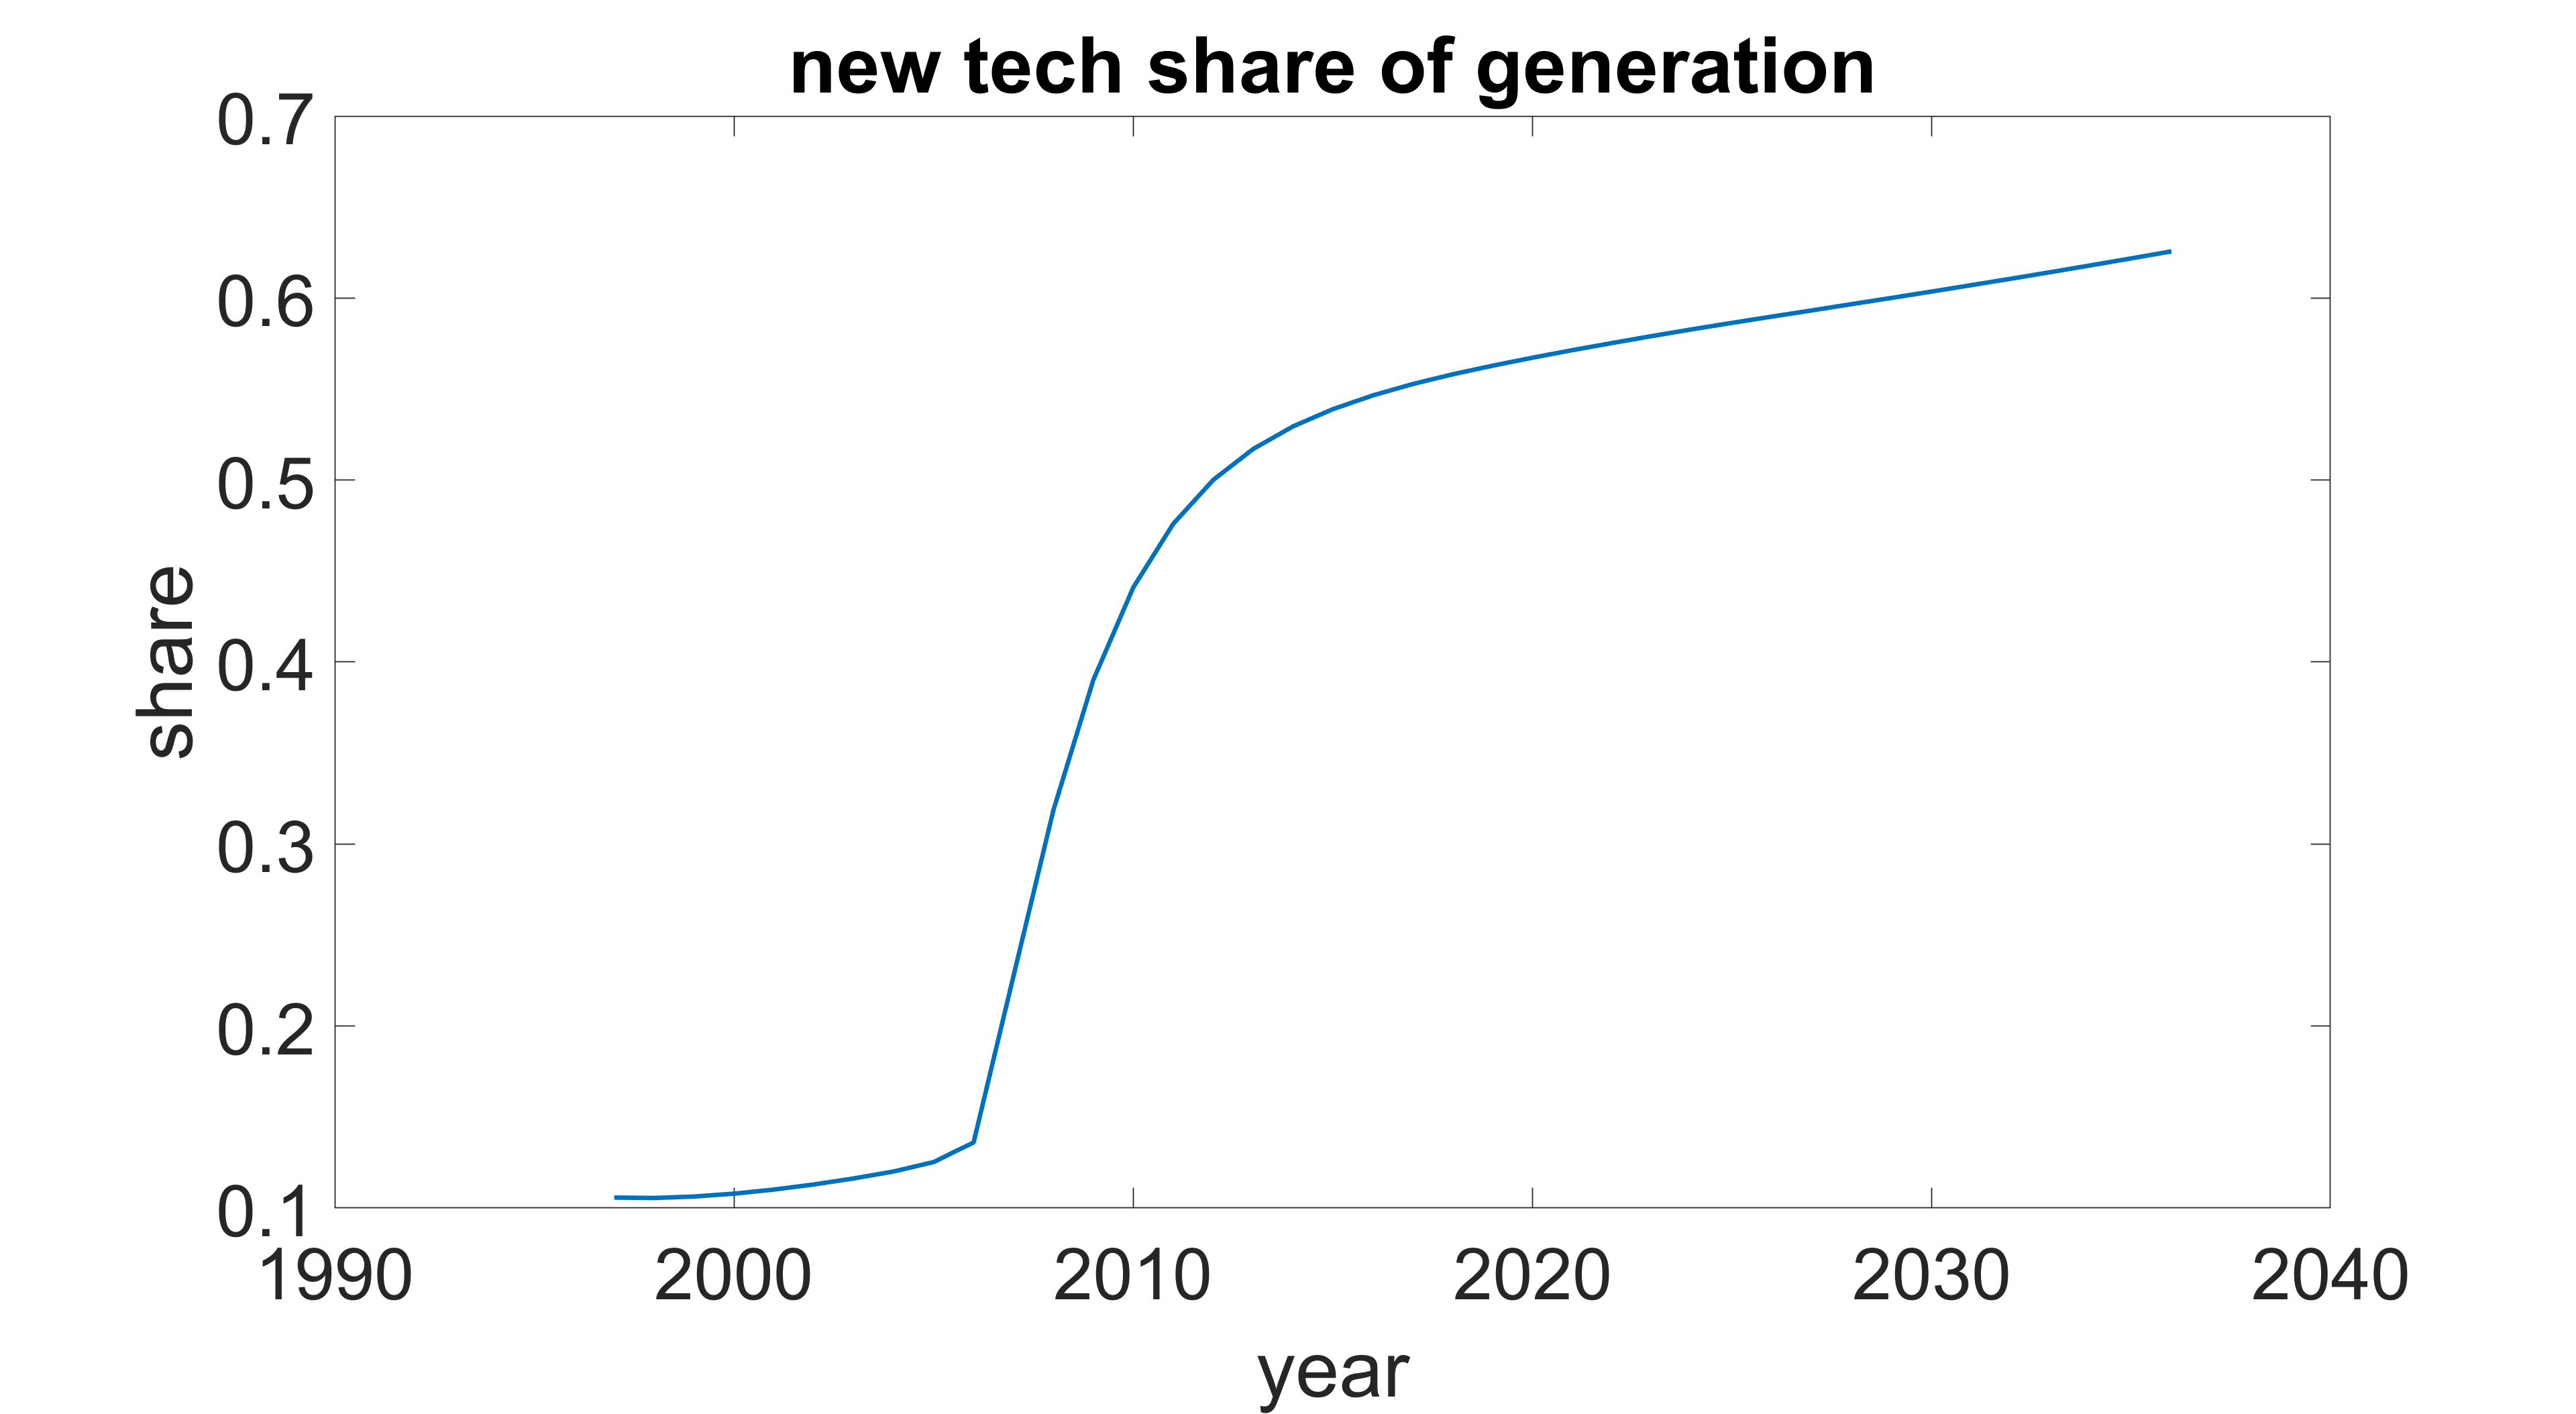
\includegraphics[scale=0.1]{share path2.png}
\end{figure}

\hyperlink{transition0}{\beamerbutton{Generation shares}}
\end{frame}

%%%%%%%%%%%%%%%
\begin{frame}{Transition 1: Coal to natural gas}\label{transit_NGprice}

\begin{figure}
\centering
\caption{Gas price over the convergence path}
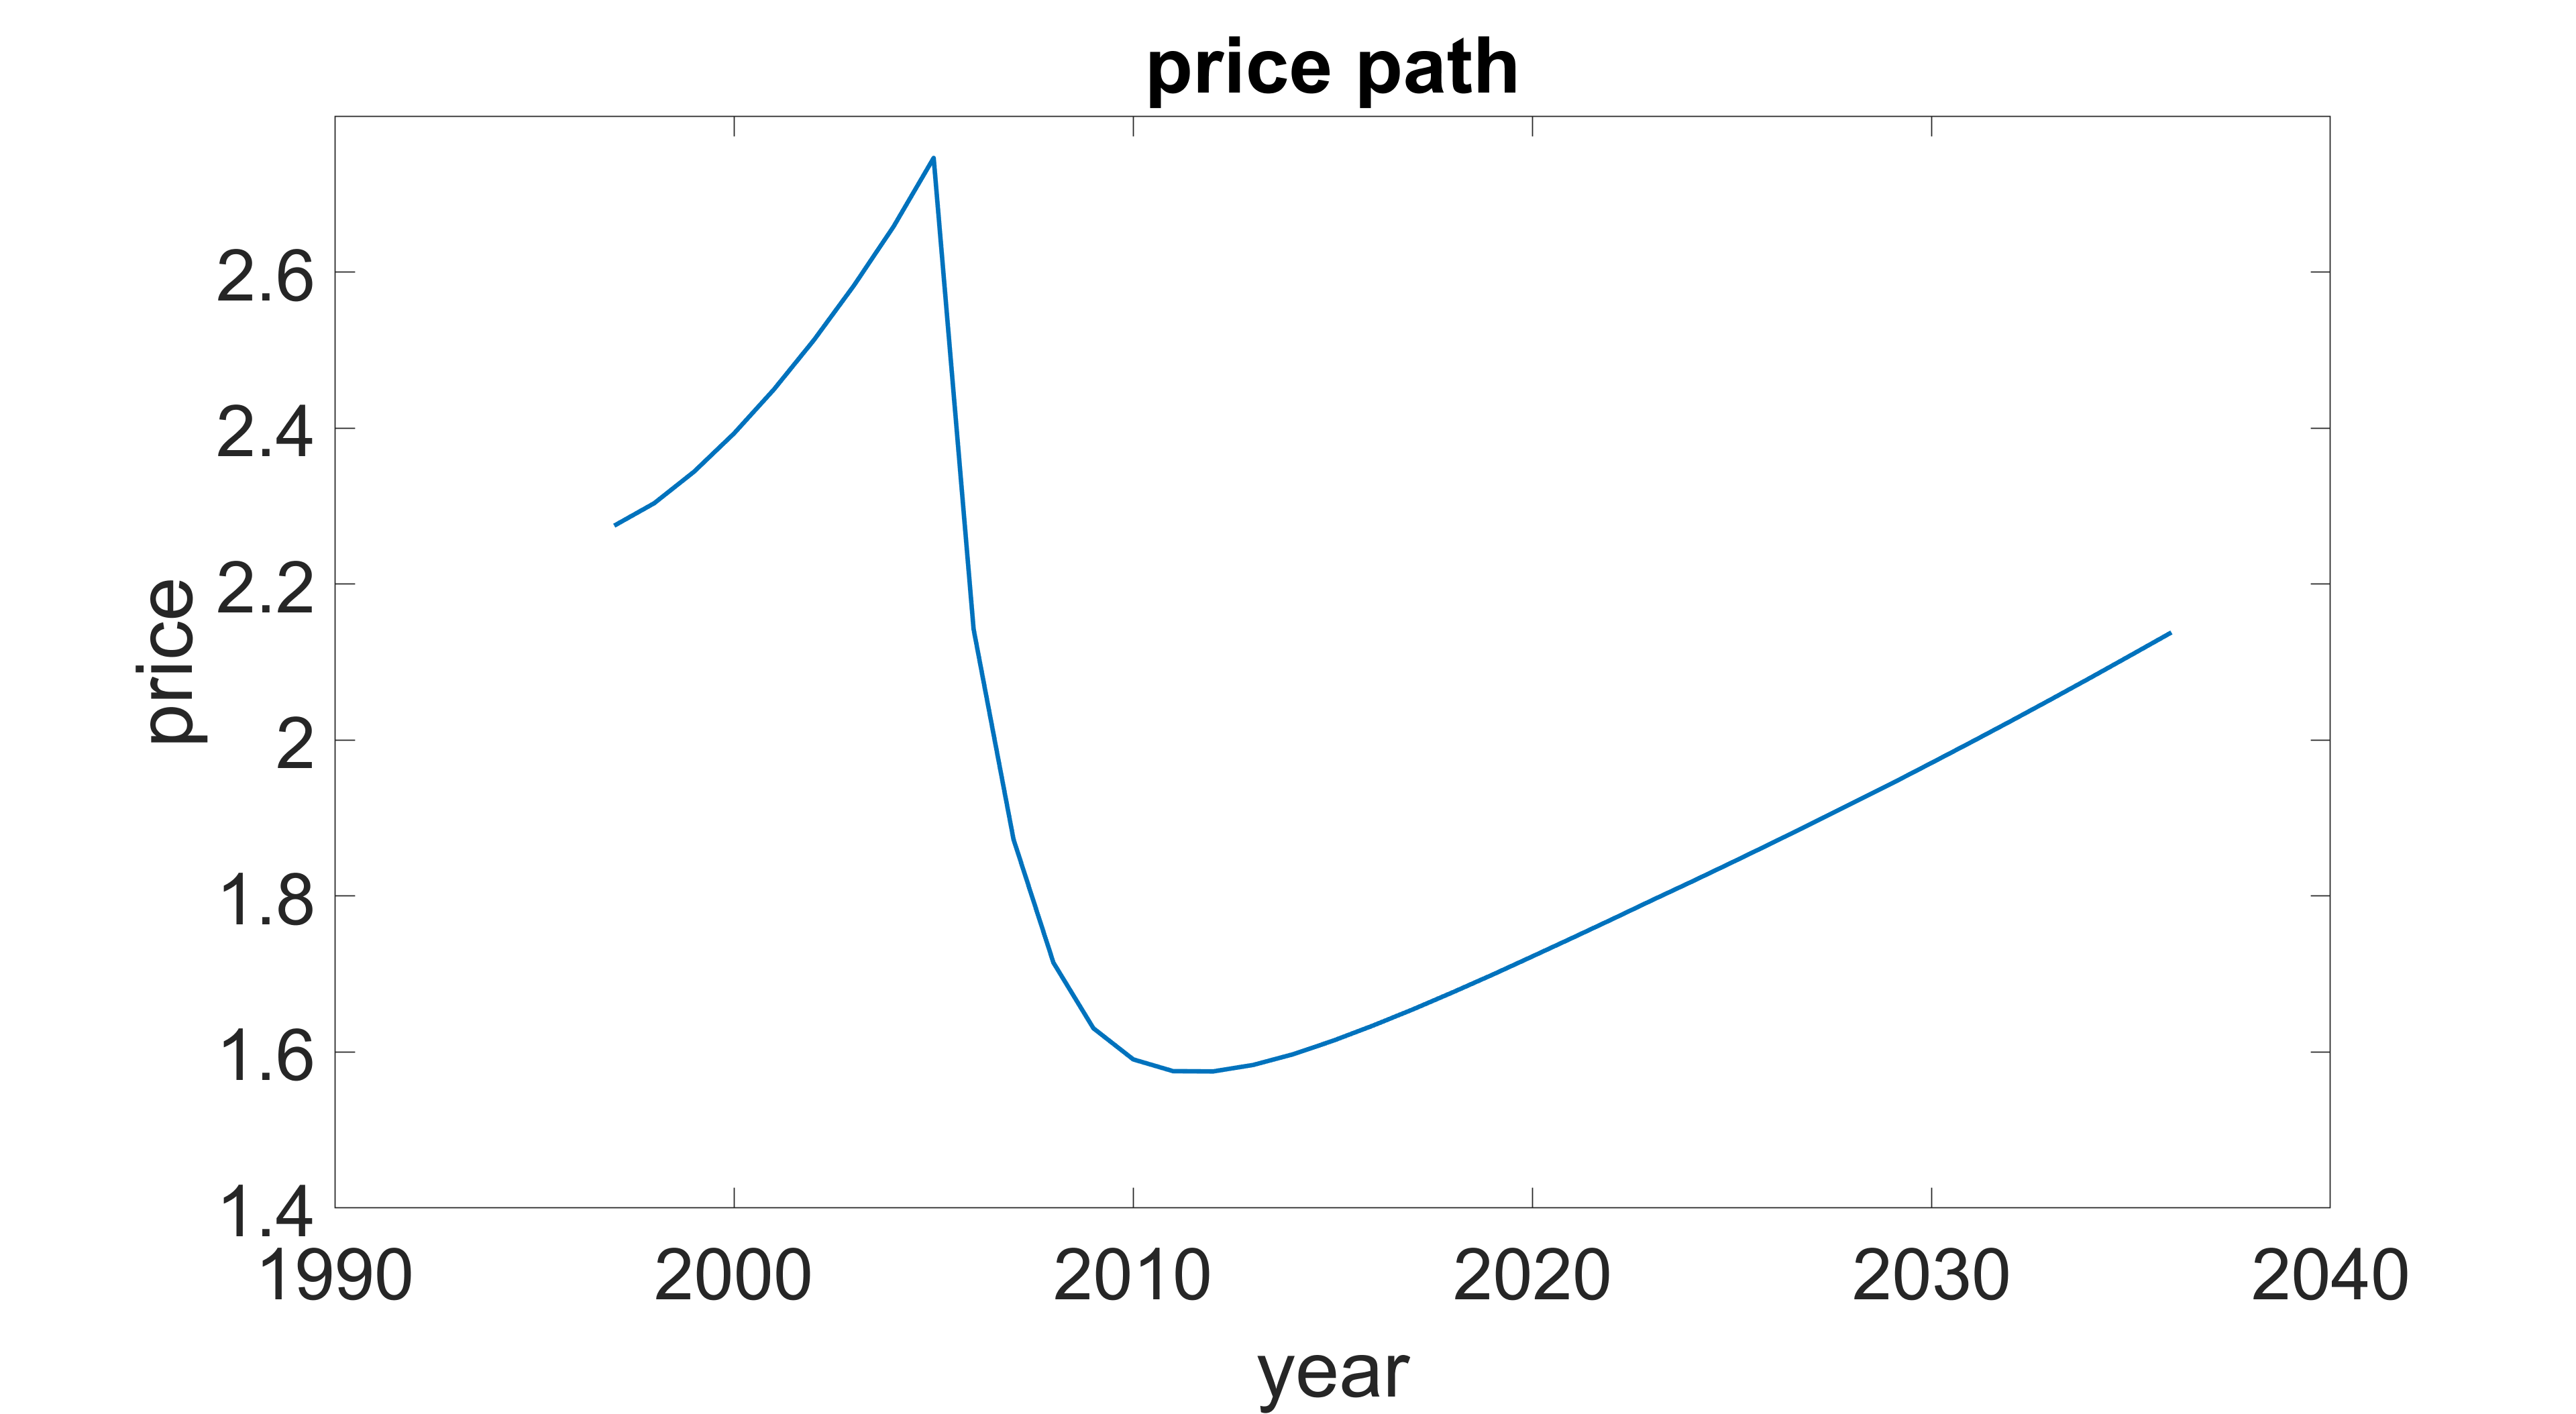
\includegraphics[scale=0.1]{gas price path.png}
\end{figure}
\hyperlink{gasindata}{\beamerbutton{Natural gas/coal cost}}
\end{frame}

%\begin{frame}{Transition 2: Coal to natural gas}

%ADD electricity price path


%\end{frame}

%%%%%%%%%%%%%%%%%%%%%%%%%%%%


\begin{frame}{Next steps: policies}
\small
\begin{itemize}
\item Federal policies
\begin{itemize}
 \item Federal support to renewable energy was estimated at  \$15.6 billion in 2022, up from \$1,417 million in 1999: mostly from a production tax credit
 
 .
 \item Support for natural gas and coal is much lower and has not increased.
\end{itemize}
 \end{itemize}
 \begin{itemize}
 \item State-level policies
 \begin{itemize}
     \item CO2 emission trading in California and ten Northeastern states
     \item Renewable portfolio standard (RPS)
     \item Feed-In Tariff Programs
 \end{itemize}
 
 \end{itemize}
 

\end{frame}
%%%%%%%%%%%%%%%

\begin{frame}{Next steps}
\begin{itemize}
    \item Find a way to calibrate the impacts of US power sector policies
    \item Calibrate and solve the second transition towards solar and wind
    \item Counterfactual analysis
    \begin{itemize}
        \item The impact of subsidies to solar and wind
        \item The level of a carbon tax with comparative impact
    \end{itemize}
\end{itemize}

\end{frame}
%%%%%%%%%%%%%%%%%

\begin{frame}[allowframebreaks]{References}
\tiny
    \bibliography{bibliography}
\end{frame}


%%%%%%%%%%%%%%%%%%%%%%%%%%%%%%%%%%%%%%%%%%%%%%%%%%%%%%%




%%%%%%%%%%%%%%%%%%%%%%%%%%%%%%%%%%%%%%%%%%%%%%%%%%%%%%%
\appendix
\section*{Appendix}


%%%%%%%%%%%%%%%
\begin{frame}{Definitions}\label{definitions}

\begin{itemize}
 \item The unit of our model is a power generator: an electricity production unit such as a natural gas steam turbine or a wind turbine.
 \item The size of a generator is not uniform.
 \item A power plant is a cluster of one or more generators and auxiliary equipment.
 \item A power sector firm may own several power plants.
 \item We assume perfect competition so generator decisions are independent of which power plant and firm they belong to.
\end{itemize}
\hyperlink{model_struct}{\beamerbutton{Model structure}}   
    
\end{frame}
%%%%%%%%%%%%%%%
\begin{frame}{Intra-period problem}\label{intra_period}
\footnotesize
    From solving the generator intra-period problem we get:\\
    \begin{align*}
        e_i^* = (\frac{a_{i,t}p_E\alpha}{p_e})^\frac{1}{1-\alpha}
    \end{align*}
    where \begin{align*}
        a_{i,t}=\frac{a_{i}^{1+\gamma t}}{(1+g_a)^t}
    \end{align*}
    \begin{itemize} 
        \item In the data $a_{i,t}$ is the relative efficiency of the generator
        \item From the generator's perspective it faces the same problem if its own efficiency depreciates or if other generators' efficiency grows with rate $1+g$  
        \item The latter implies that market base demand grows with rate $(1+g)^\frac{1}{1-\alpha}$
        \item We therefore incorporate depreciation and growth in the average productivity of the market in the same depreciation term
    \end{itemize}
    
 \hyperlink{gen_problem}{\beamerbutton{Generator problem}}    
\end{frame}

%%%%%%%%%%%%%%%
%%%%%%%%%%%%%%%
\begin{frame}{Alternative model setup}\label{alt_model}
\footnotesize
\begin{itemize}
    \item We could also set up a generator problem with a CRS function where the average price that a generator observes is declining in production
    \item This is due to daily variation in electricity prices and the imperfect substitutability of generators
    \item As a generator increases its production this will occur at times with lower electricity prices $p_E$. The average price that the generator observes is:
\end{itemize}   
    \small\begin{align*}
        p_E(e_i) = p_0e_i^{-\eta}
    \end{align*}
    \small The period problem becomes:
    \small\begin{align*}
        \max_{e_i} a_{i,t}e_ip_E(e_i) - p_ee_i \rightarrow e_i^* = (\frac{p_0a_{i,t}(1-\eta)}{p_e})^\frac{1}{\eta} \\\implies \alpha = 1-\eta , p_E = p_0\frac{\eta}{1-\eta} \text{ equalizes the two settings}
    \end{align*}
    \hyperlink{gen_problem}{\beamerbutton{Generator problem}}   
\end{frame}
%%%%%%%%%%%%%%%%%%%%%%%%%%%%%%%%%%%%%%%%%

\begin{frame}{The model: switch from coal to gas}\label{coal_gas}
\footnotesize
\begin{itemize}
    \item Some fossil fuel generators can be converted from using one fuel to another
    \item In the coal-gas transition we allow coal generators to switch to natural gas by paying a switching cost
    \item The generator keeps it's initial productivity adjusted by the productivity gap between coal and natural gas
\end{itemize}
\begin{align*}
    v_{c,conv}(a_i,t) = \max \big\{ v_c(a_i,t), v_g(\frac{a_i}{(1+\Delta_g)^{\Delta_t}},t)-c_{conv}\big\}
\end{align*}
Where $\Delta_g$ is the difference between the growth rate of gas and coal efficiency idiosyncratic distributions and $\Delta_t$ is the number of years this differential growth rate has been in place. \\\\
\hyperlink{gen_problem}{\beamerbutton{Period problem}}    
\hyperlink{value_fn}{\beamerbutton{Value function}}    

\end{frame}
%%%%%%%%%%%%%%%
\begin{frame}{Why relative efficiency matters}\label{rel_eff_why}
\footnotesize
\small\begin{itemize}
    \item Let's assume that the generators depreciate with rate $g_0$ and the distribution of the newcomers' efficiency is growing with the rate $g_n$
    \item $c_f$, $c_a$ should also grow with the rate $g_n^\frac{1}{1-\alpha}$: otherwise they become negligible compared to operating costs, as profits are given by:\\
    %
\end{itemize}
\begin{align*}
        \pi_{ent,t+\hat{t}}(a_j) &= \left(\frac{p_E a_j\left(1+g_n\right)^\hat{t}}{p_e^\alpha}\right)^{\frac{1}{1-\alpha}} \frac{1-\alpha}{\alpha} - c_{f,t}\\
        \pi_{update}(a_i,t) &= \left(\frac{p_E a_i^{1+\gamma (t-\tau)}}{p_e^\alpha\left(1+g_0\right)^{(t-\tau)}\left(1+g_n\right)^\tau}\right)^{\frac{1}{1-\alpha}} \frac{1-\alpha}{\alpha}-c_{f,t}, \\\\ \quad (\tau>t \rightarrow \tau = t)
    \end{align*}
\end{frame}

%%%%%%%%%%%%%%%%

\begin{frame}{Why relative efficiency matters}\label{rel_eff2}
\footnotesize
    \begin{itemize}
        \item This means unless $c_{f,t}$ is growing with the rate $g_n^\frac{1}{1-\alpha}$, in the long term it has a negligible effect on the firm's profit. 
        \item The profits of the updating and entrant firms grow at rate $g_n$. This implies that $c_{a,t}$ must grow at the rate $g_n^\frac{1}{1-\alpha}$ for there to be a stable solution to the firm's adoption problem
        \item $c_{e,t}$ also needs to grow at the rate $g_n$ so the mass of firms is constant in steady state.
        \item In that case we can normalize all values by the growth rate $(1+g_n)^\frac{1}{1-\alpha}$. 
        \item This means that the value of entering and adopting firm doesn't grow but the effective efficiency of non-adopting firms depreciates at the rate $1+g_a = (1+g_0)(1+g_n)$
        \item Alternatively we can set $g_n=0$ from the beginning and consider the effect of growth in absolute efficiencies
    \end{itemize}
    \hyperlink{gen_problem}{\beamerbutton{Generator problem}}
    \hyperlink{mainss}{\beamerbutton{Main model results}}
    \hyperlink{Data}{\beamerbutton{Main data results}}
    
\end{frame}

%%%%%%%%%%%%%%%%%%%


\begin{frame}{Model: Steady state results}\label{mainss}
\begin{figure}
\centering
\caption{Coal power plants: efficiency distribution before transition}
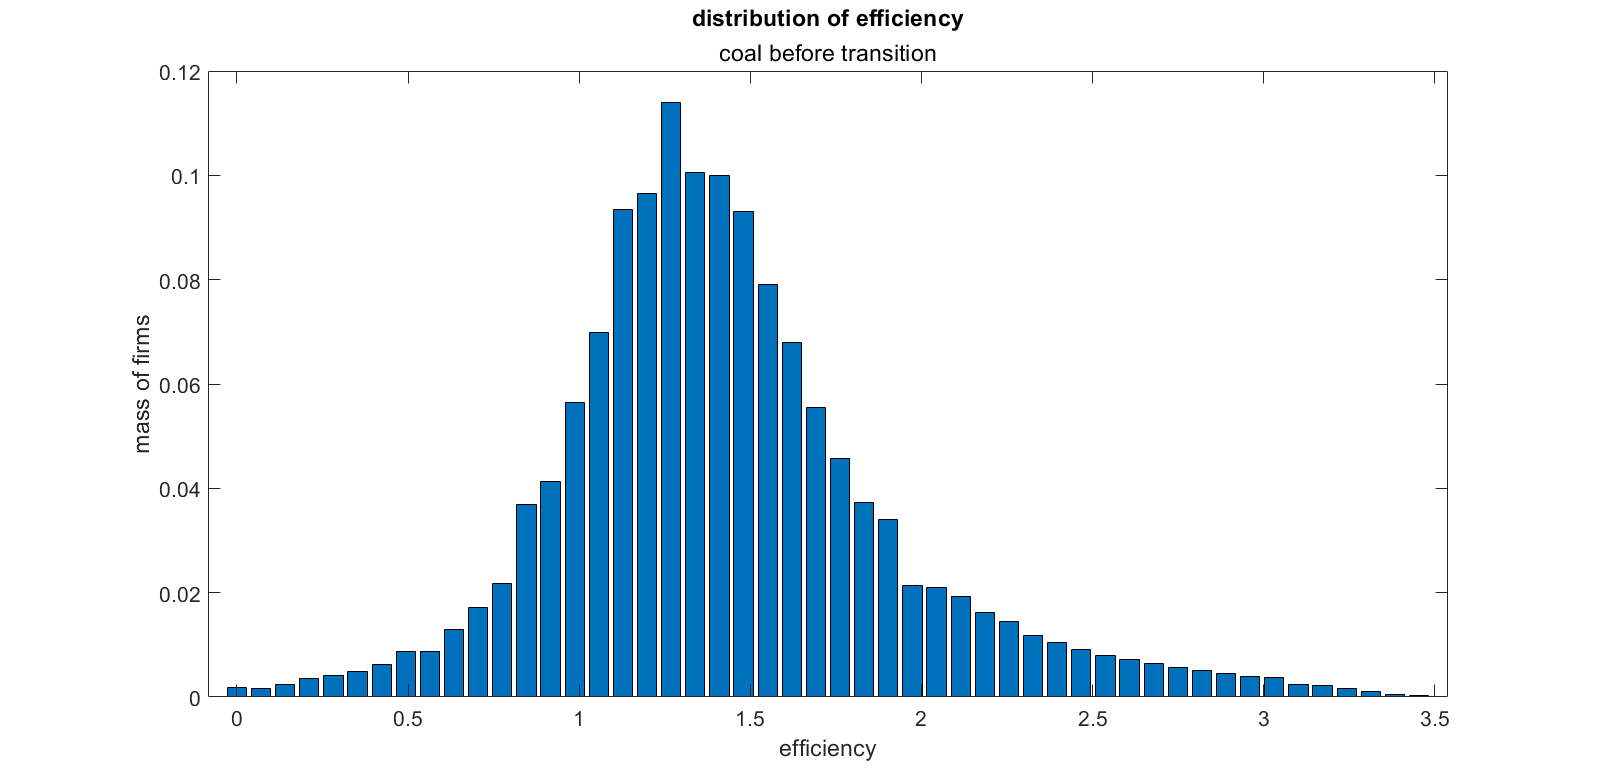
\includegraphics[scale=0.25]{power plant efficiency dist (coal before).png}
\end{figure}
\hyperlink{moress}{\beamerbutton{More ...}}
\end{frame}

%%%%%%%%%%%%%%%%

%%%%%%%%%%%%%%%%%%%%%%
\begin{frame}{Model: Steady state results}\label{moress}
\begin{figure}
\centering
\caption{Coal power plants: technological age distribution before transition}
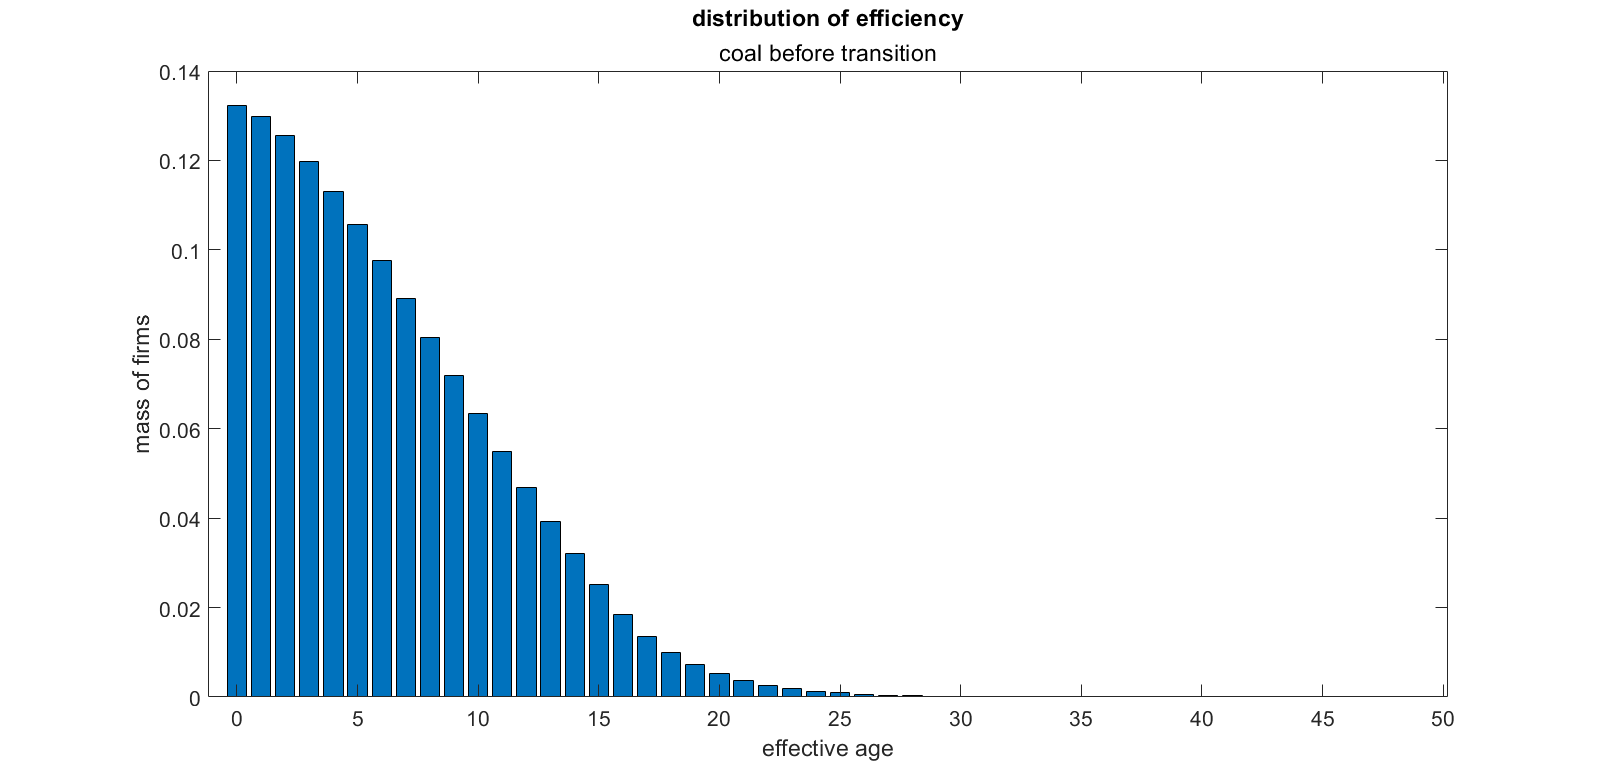
\includegraphics[scale=0.25]{power plant age dist (coal before).png}
\end{figure}
\hyperlink{mainss}{\beamerbutton{Main results}}
\end{frame}

%%%%%%%%%%%%%%%%
\begin{frame}{Model: Steady state results}
\begin{figure}
\centering
\caption{Coal power plants: likelihood of technological update}
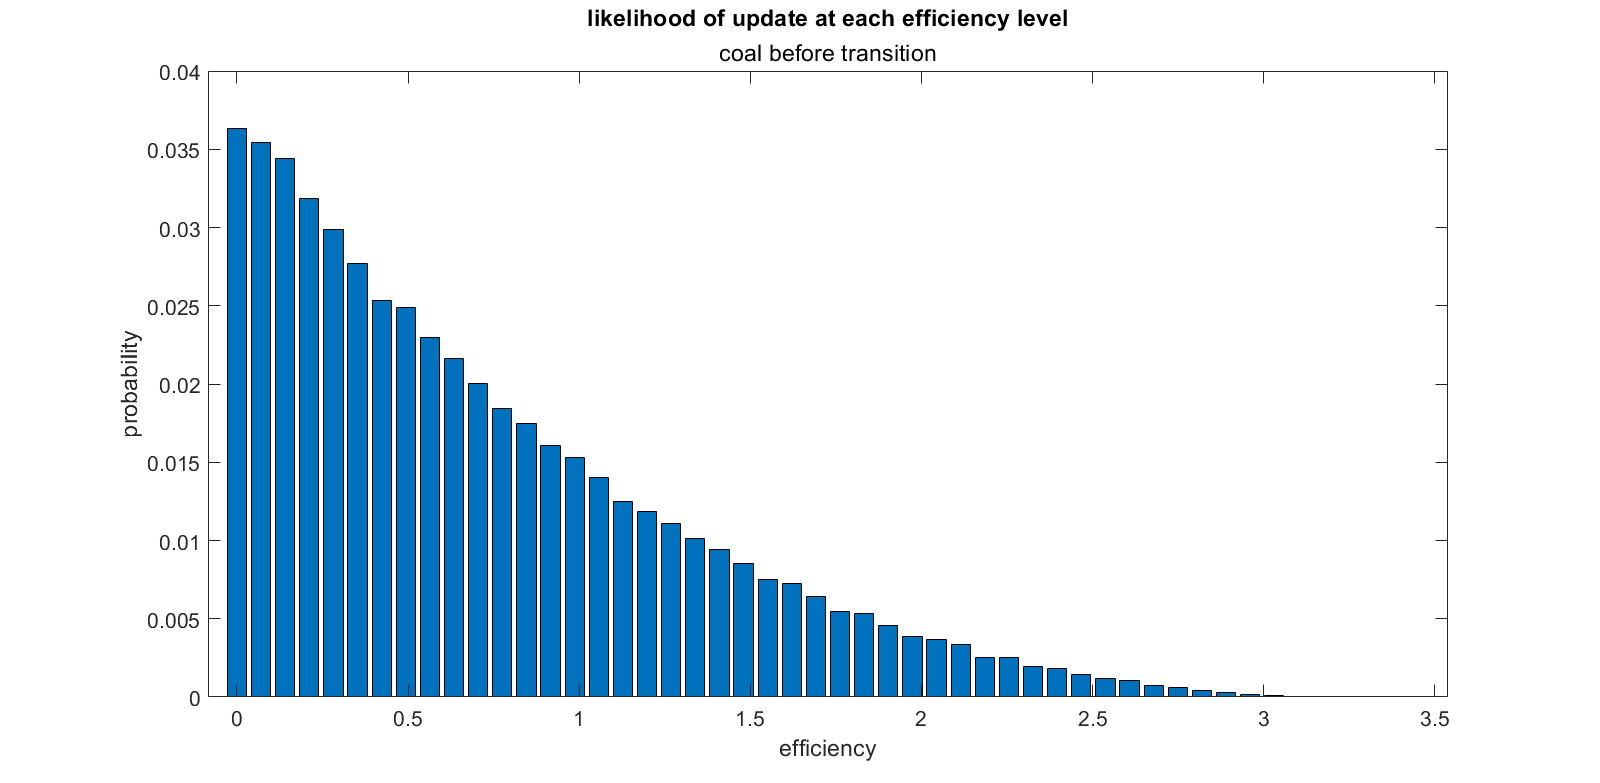
\includegraphics[scale=0.25]{update_coal_1st.png}
\end{figure}
\hyperlink{mainss}{\beamerbutton{Main results}}
\end{frame}


%%%%%%%%%%%%%%%%
\begin{frame}{Model: Steady state results}
\begin{figure}
\centering
\caption{Conventional power plants: probability of technology adoption before transition}
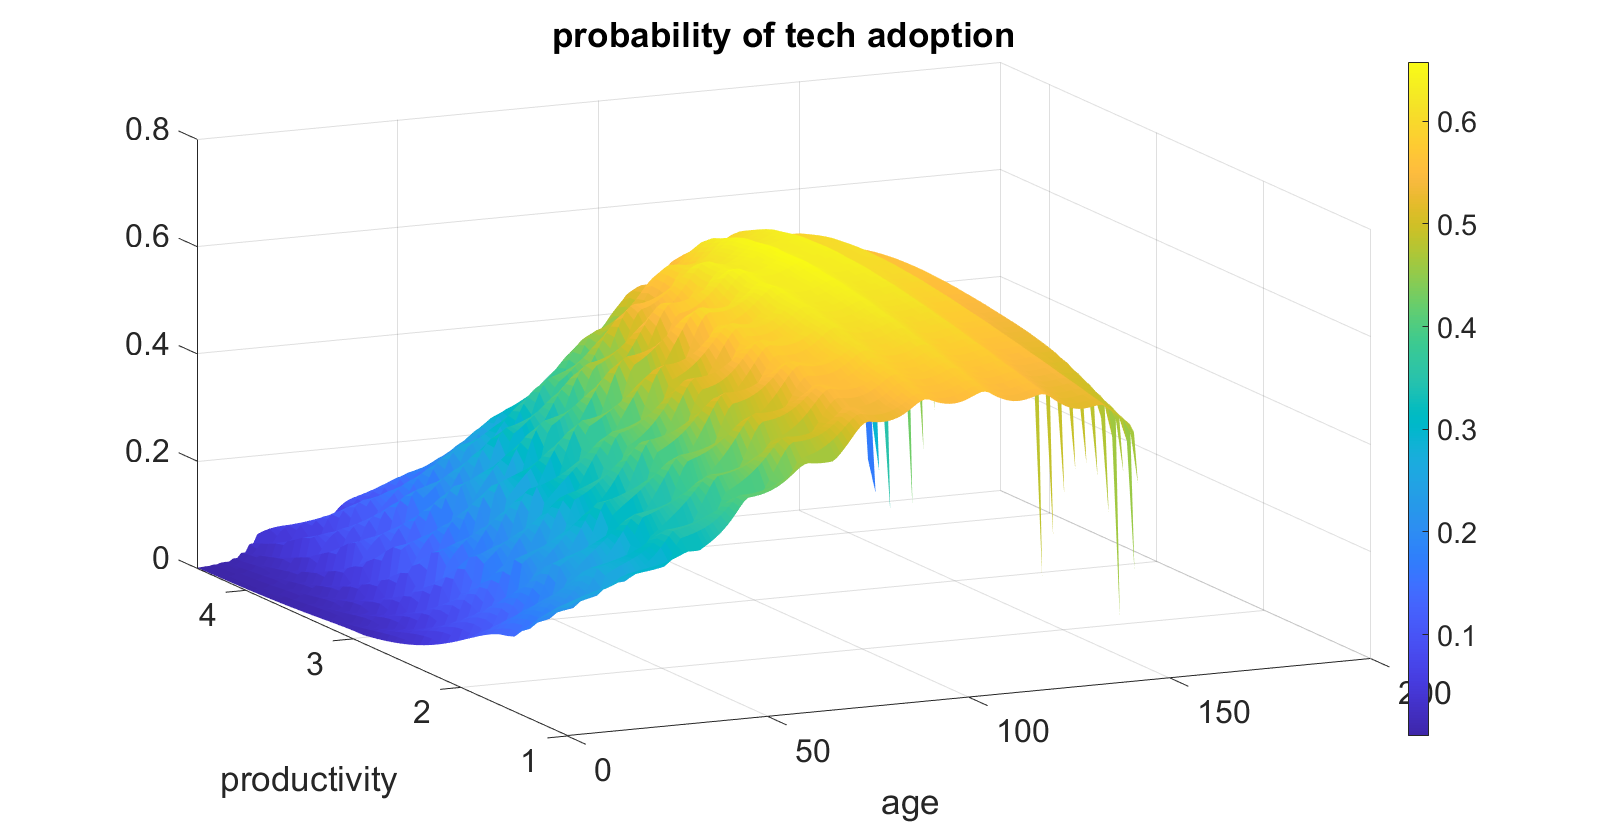
\includegraphics[scale=0.25]{prob_gas_before.png}
\end{figure}
\hyperlink{mainss}{\beamerbutton{Main results}}
\end{frame}

%%%%%%%%%%%%%%%%

\begin{frame}{Model: Steady state results}
\begin{figure}
\centering
\caption{Solar and wind power plants: probability of technology adoption before transition}
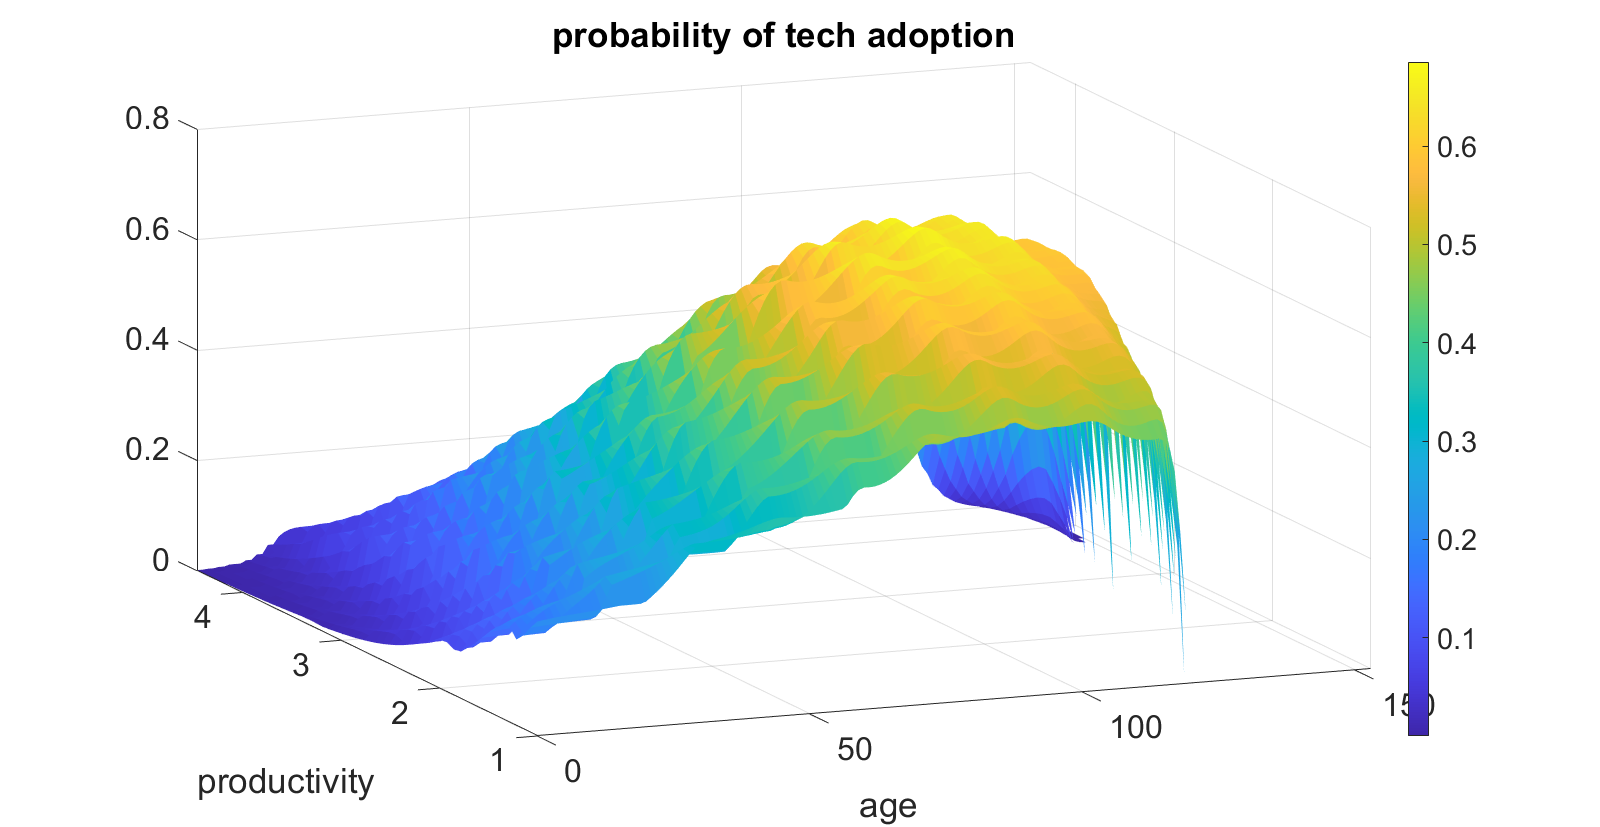
\includegraphics[scale=0.25]{prob_sola_before.png}
\end{figure}
\hyperlink{mainss}{\beamerbutton{Main results}}
\end{frame}


%%%%%%%%%%%%%%%%
%%%%%%%%%%%%%%%%
\begin{frame}{Transition 1: Conventional fuels to natural gas}
\begin{figure}
\centering
\caption{The path of shocks in the model}
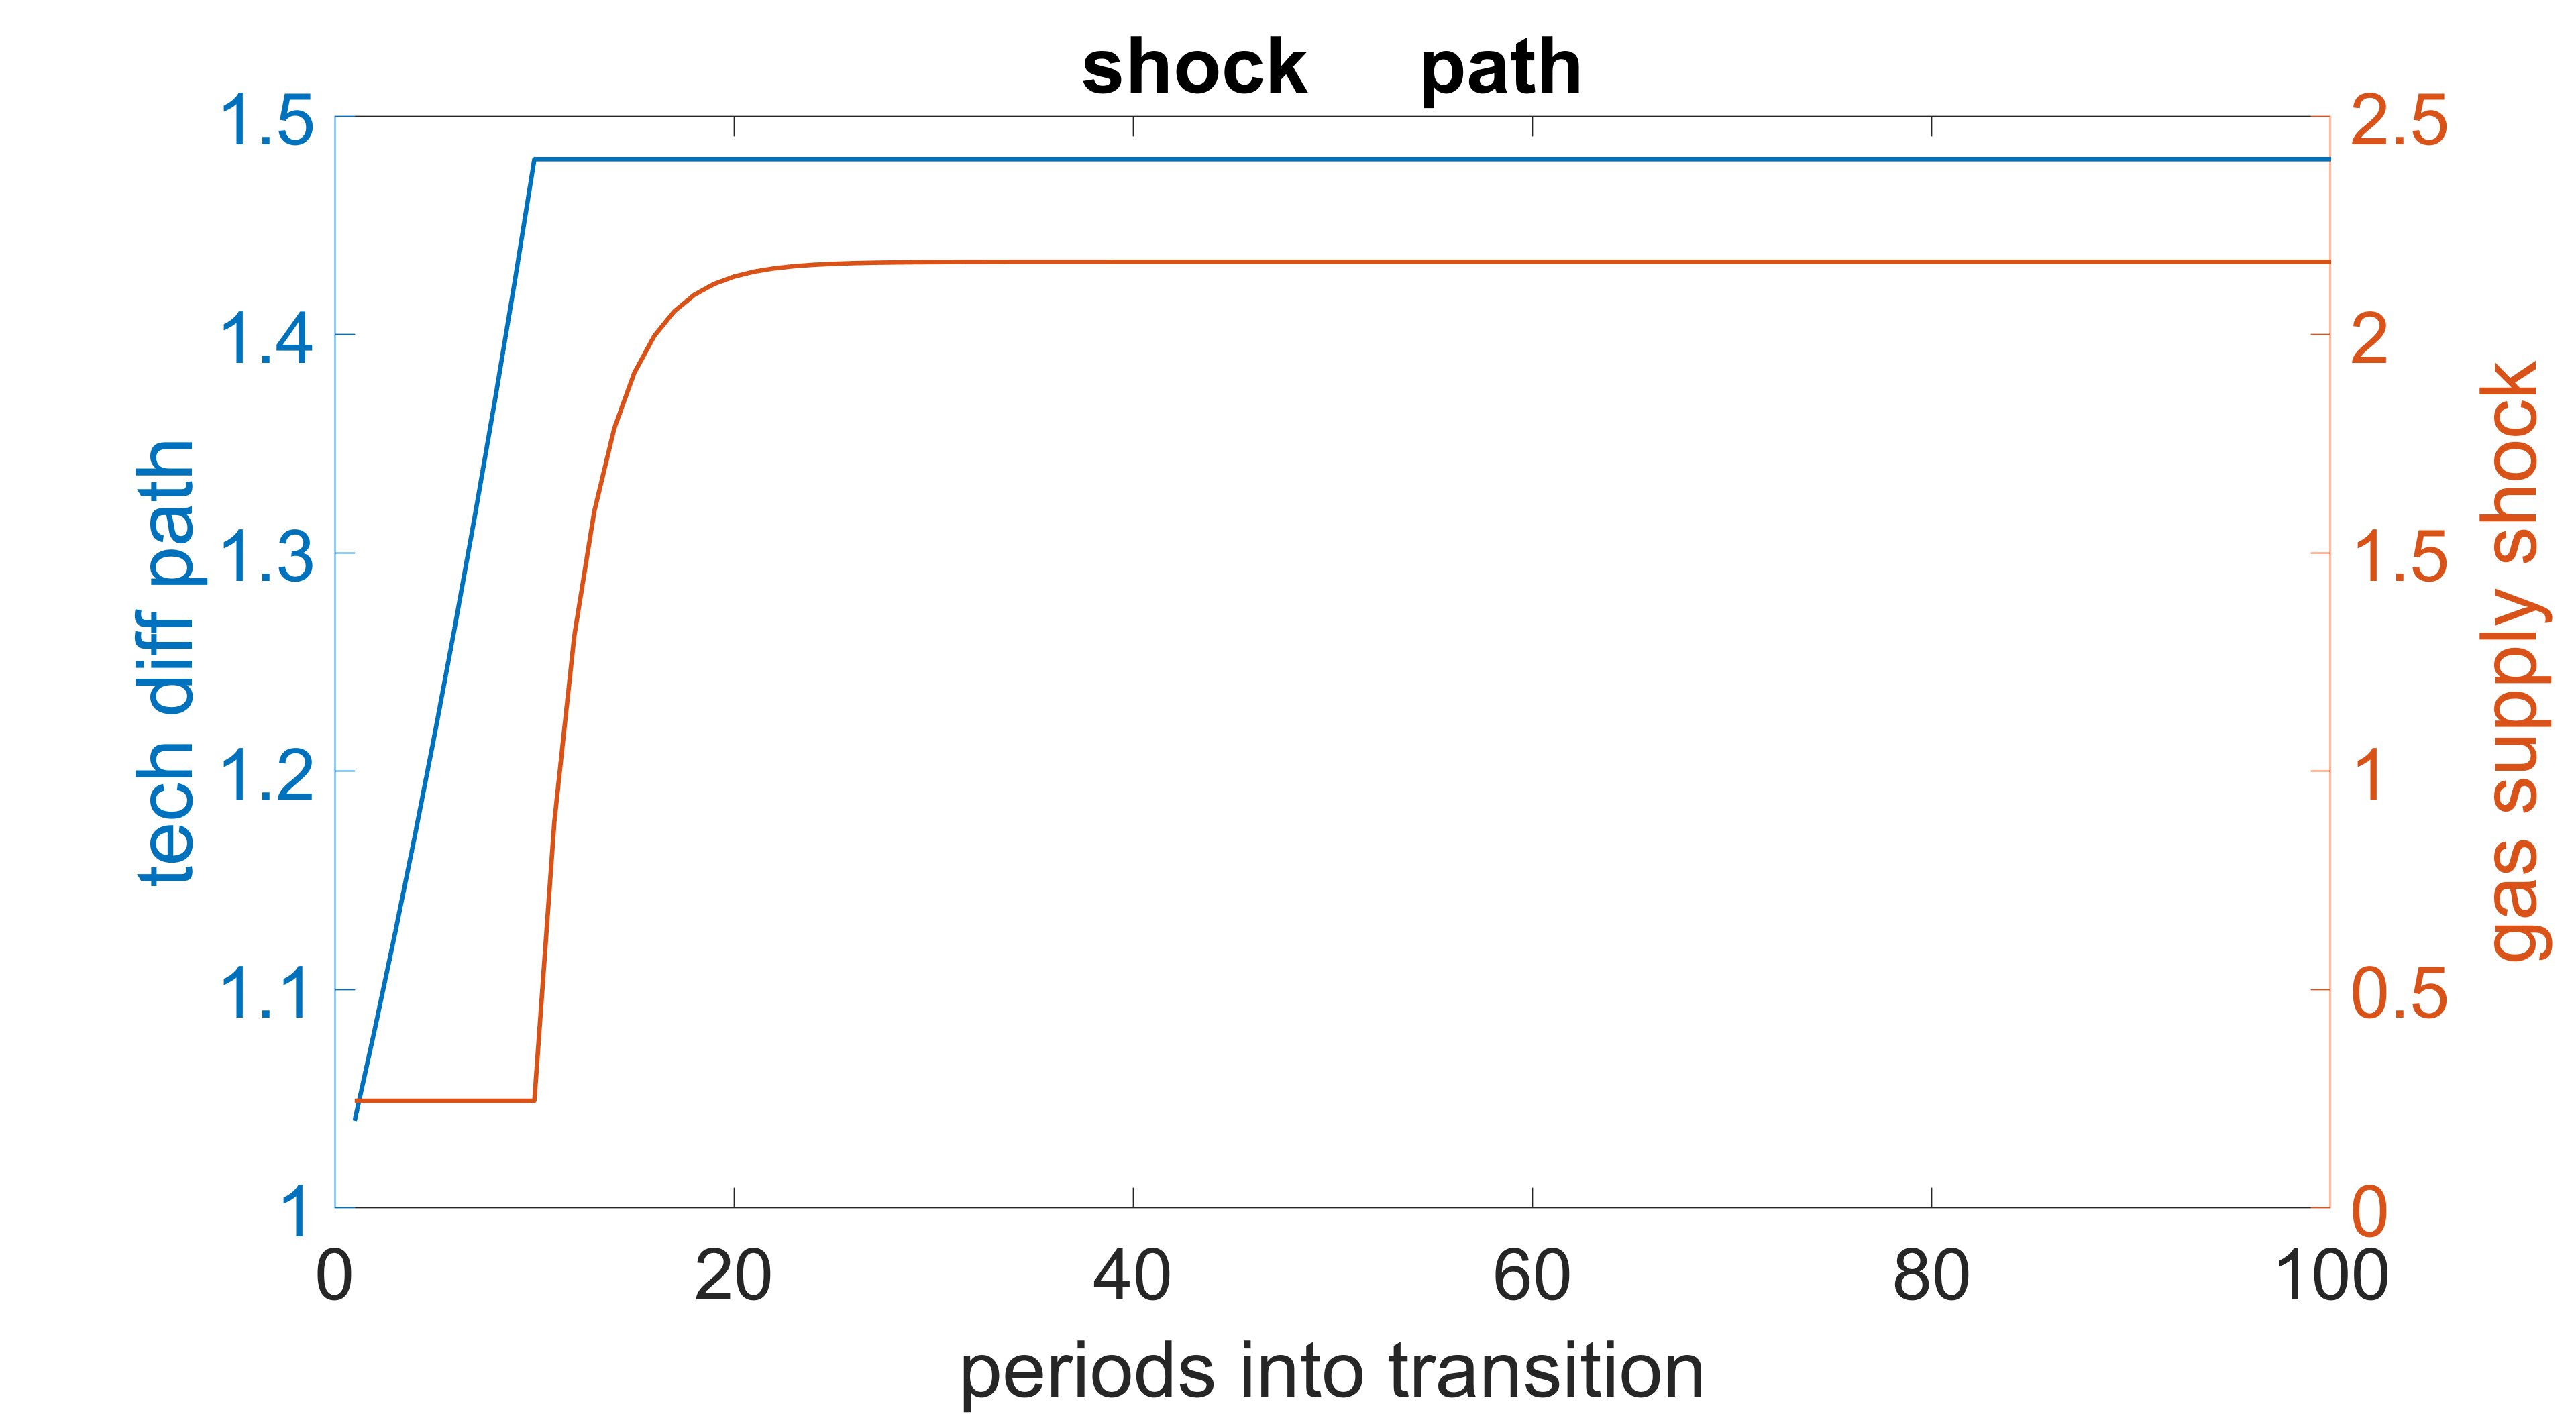
\includegraphics[scale=0.10]{shock path cg.png}
\end{figure}

\end{frame}
%%%%%%%%%%%%%%%


\begin{frame}{Transition 1: Conventional fuels to natural gas}
\begin{figure}
\centering
\caption{Share of gas generation over the convergence path}
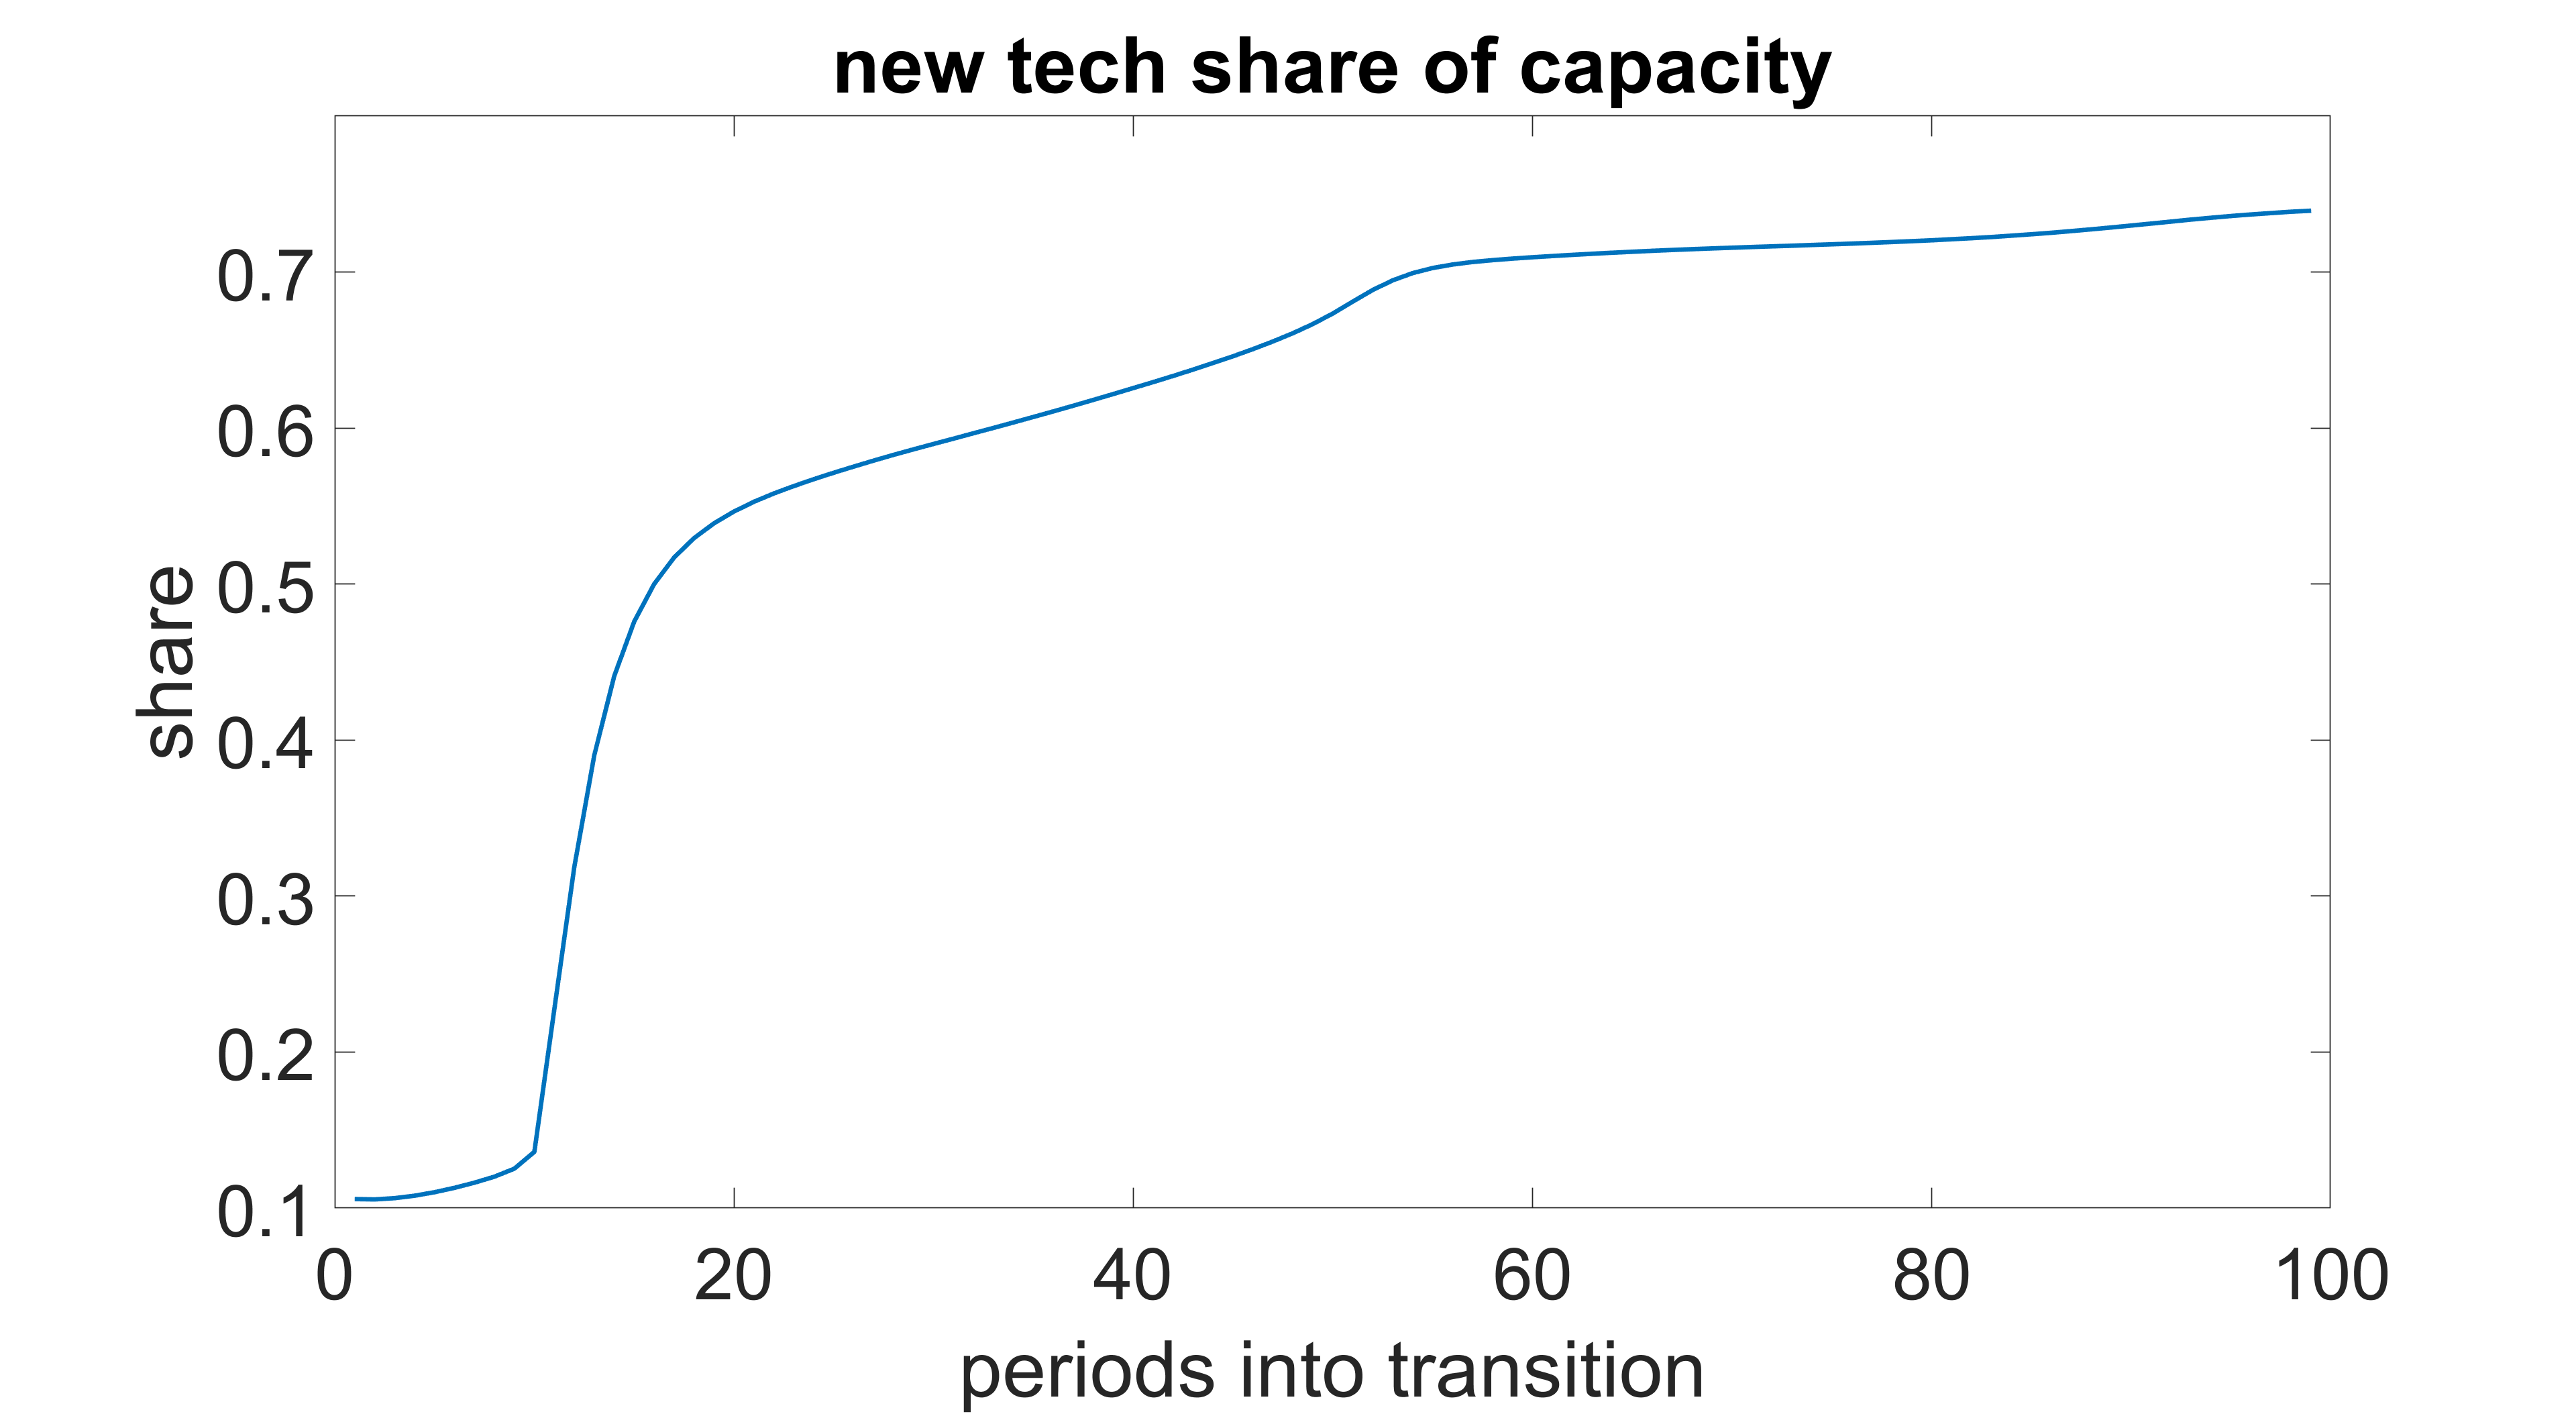
\includegraphics[scale=0.10]{share path.png}
\end{figure}

\end{frame}

%%%%%%%%%%%%%%%%%%%%%%%%%%%%%%%%%%%%%%%%%%%%%%%%%%%%%%%
\begin{frame}{Transition 1: Conventional fuels to natural gas}
\begin{figure}
\centering
\caption{Electricity price over the convergence path}
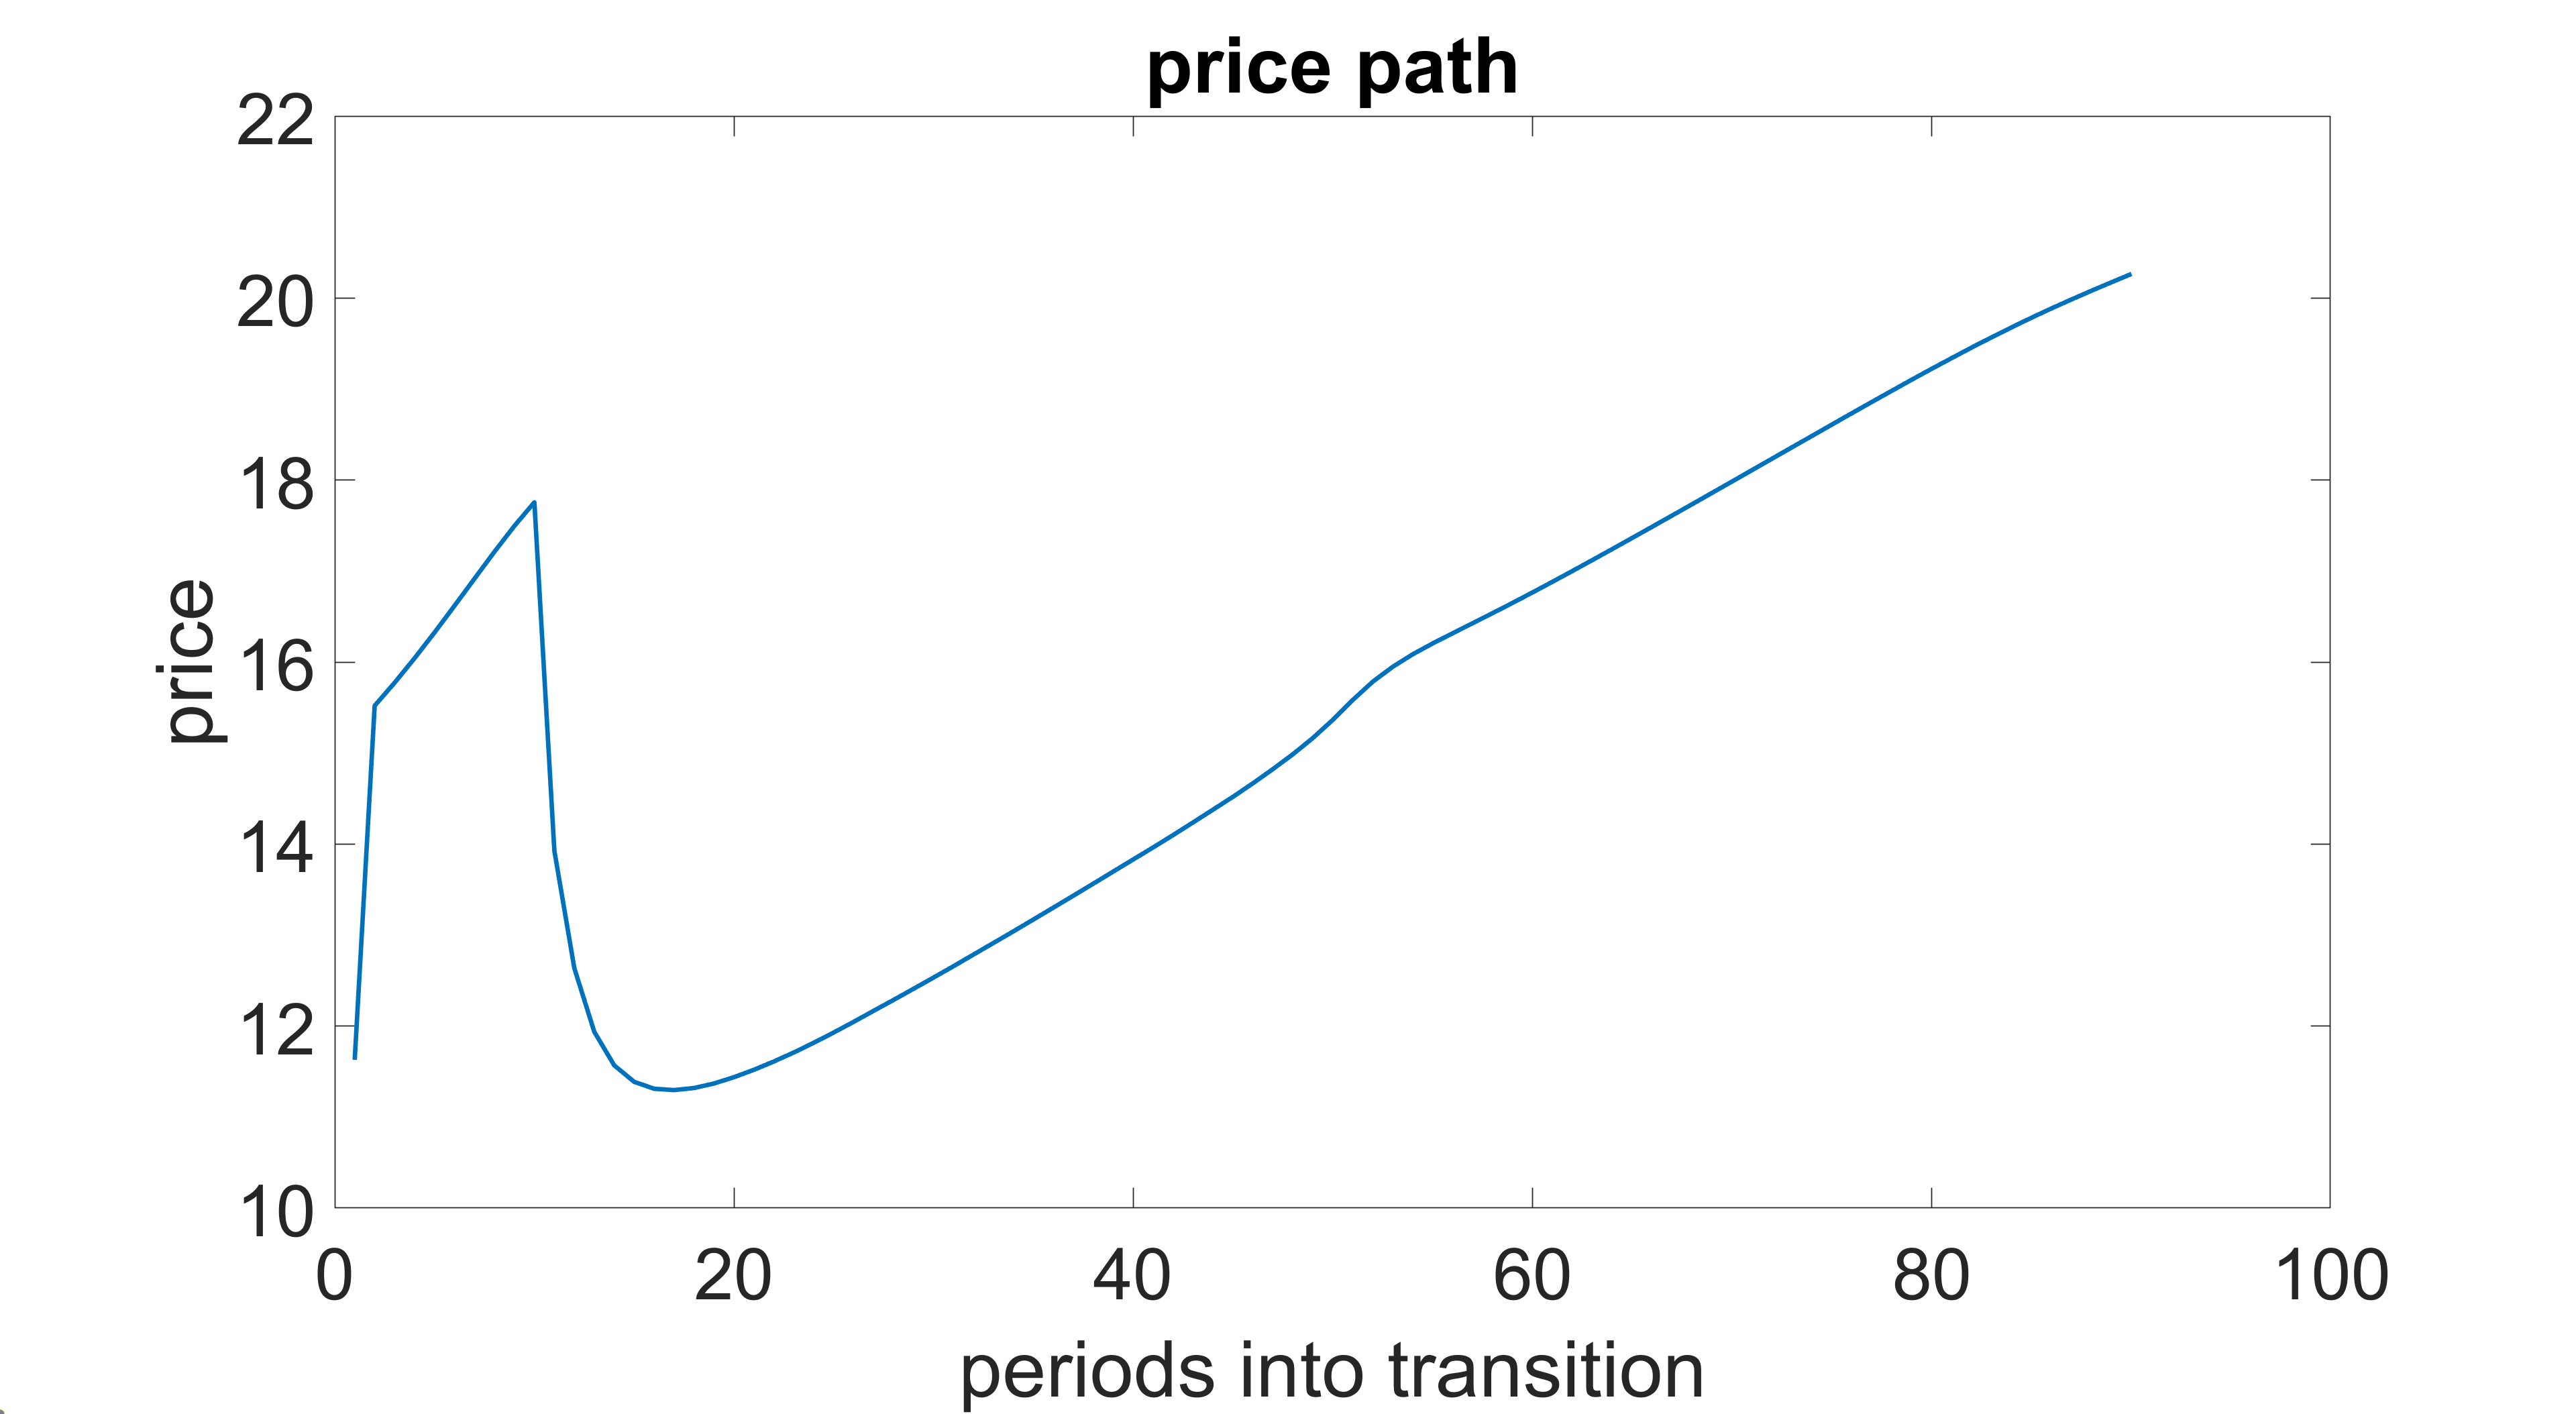
\includegraphics[scale=0.10]{price path.png}
\end{figure}

\hyperlink{transition2}{\beamerbutton{transition2}}
\hyperlink{effic_between_model}{\beamerbutton{back}}
\end{frame}

%%%%%%%%%%%%%%%

\begin{frame}{Transition 2: Conventional fuels to solar and wind}\label{transition2}

\begin{figure}
\centering
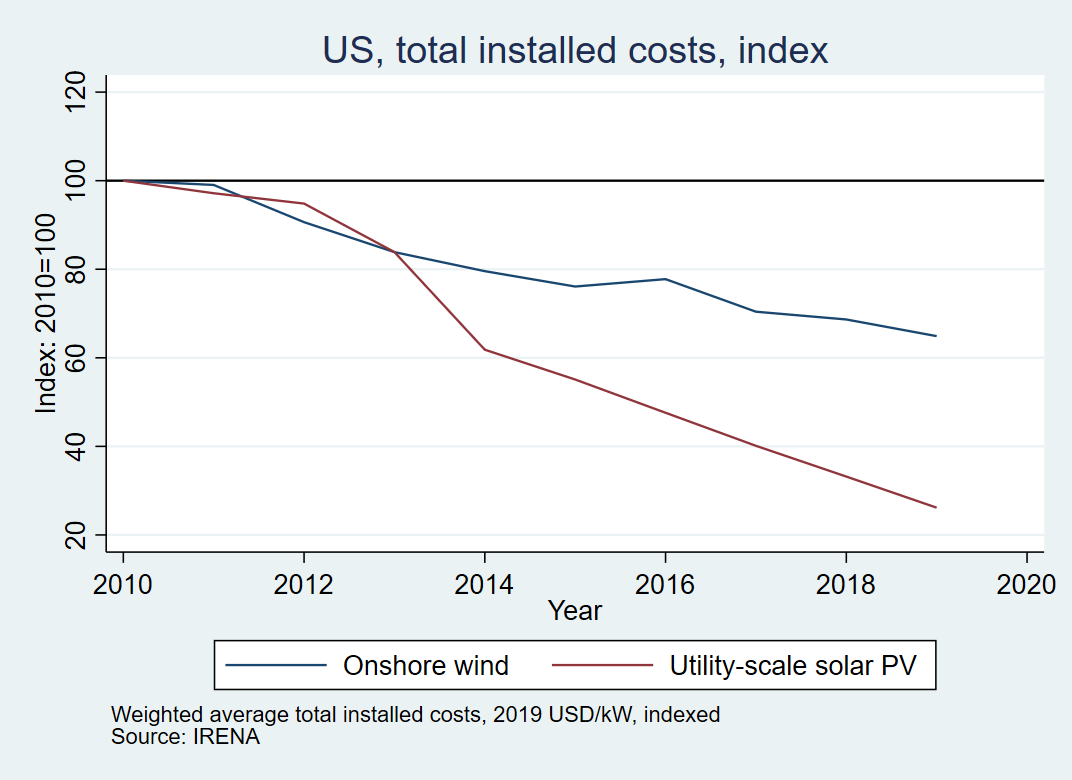
\includegraphics[scale=0.25]{solarwind_installedcosts_index.png}
\end{figure}
\hyperlink{transit_shocks1}{\beamerbutton{Transition 1}}
    
\end{frame}
%%%%%%%%%%%%%%%
\begin{frame}{Transition 2: Conventional fuels to solar and wind}
\begin{figure}
\centering
\caption{The path of installation costs in the model}
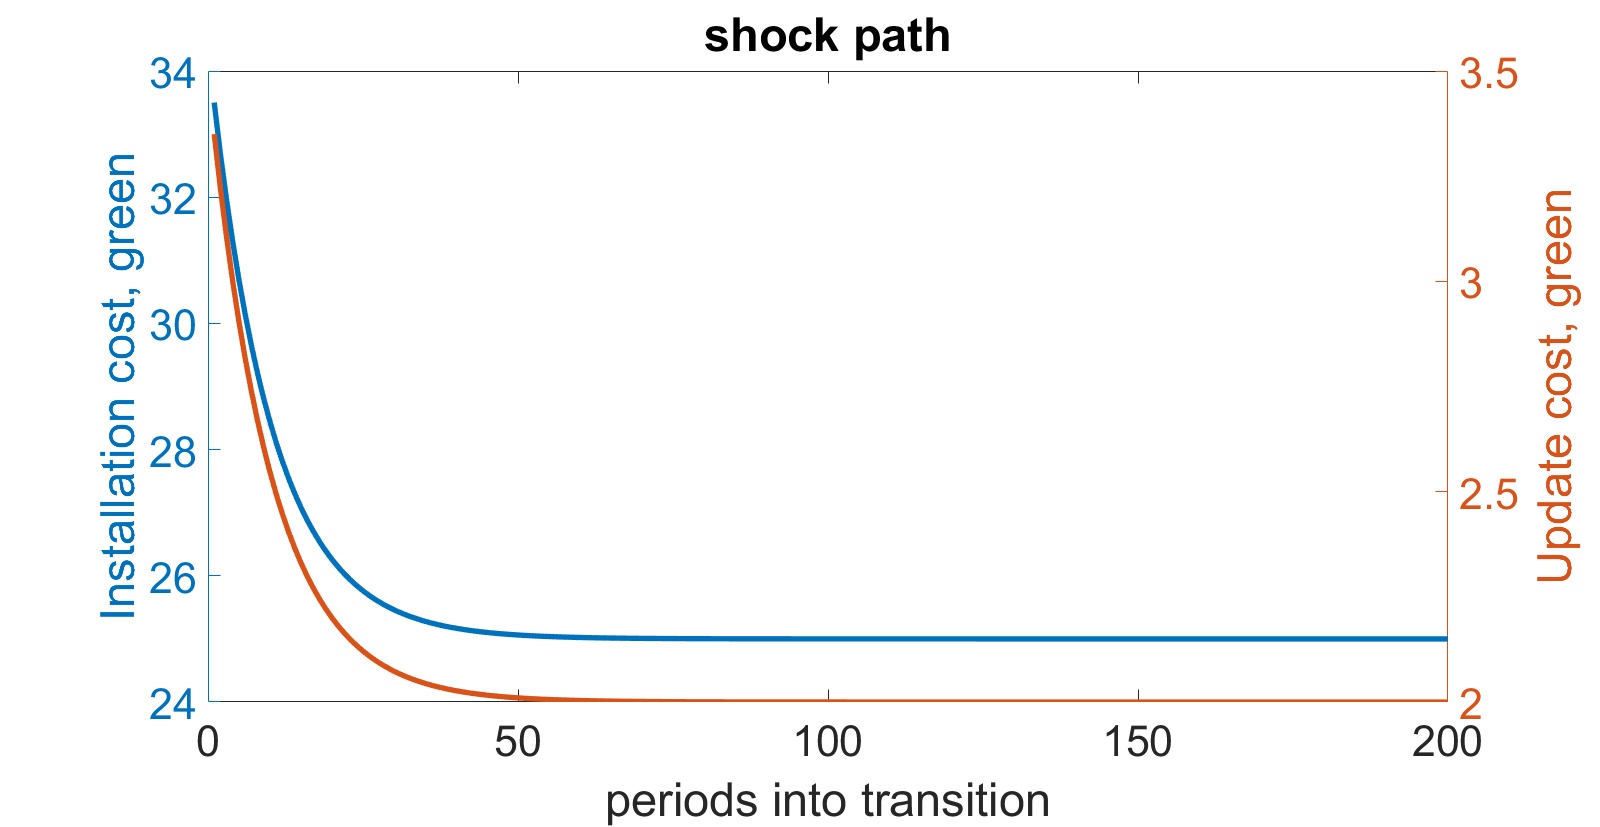
\includegraphics[scale=0.23]{shock path.png}
\end{figure}

\end{frame}
%%%%%%%%%%%%%%%


\begin{frame}{Transition 2: Conventional fuels to solar and wind}
\begin{figure}
\centering
\caption{Electricity price over the convergence path}
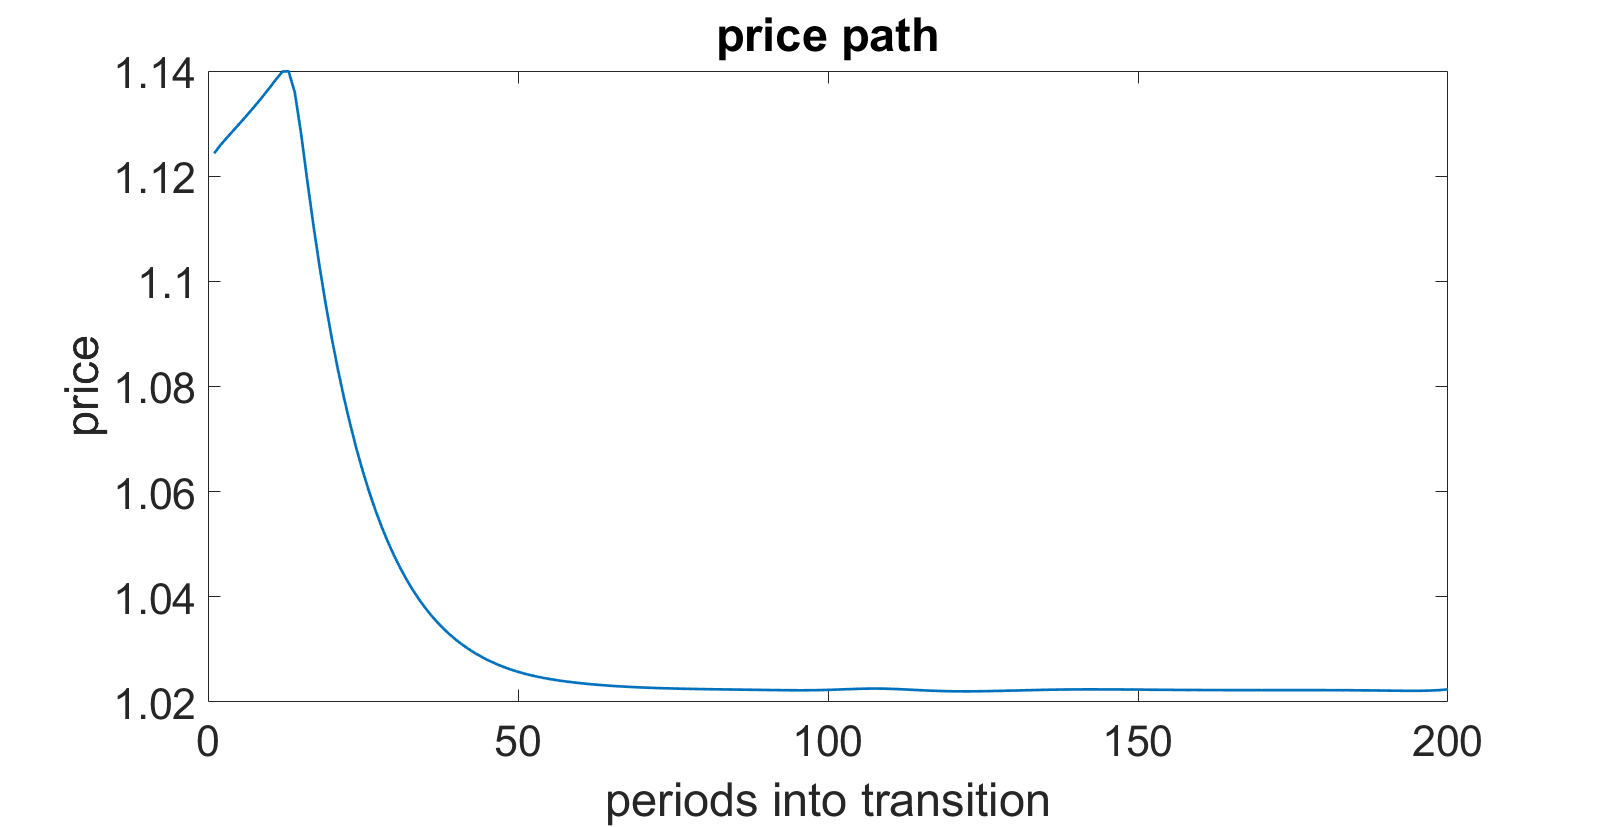
\includegraphics[scale=0.23]{price_path.png}
\end{figure}

\hyperlink{transition1}{\beamerbutton{transition1}}

\end{frame}
%%%%%%%%%%%%%%%


\begin{frame}{Data: Adoption patterns}\label{patterns_all}
\footnotesize
\begin{table}
\centering
\caption{Technology adoption dummy regressed on covariates, all plants}
\scriptsize
\begin{tabular}{lcc} \hline
 & (1) & (2) \\
VARIABLES & Raw data & Fixed effects \\ \hline
 &  &  \\
Relative efficiency after latest upgrade & -0.0701*** & -0.268*** \\
 & (0.00653) & (0.0430) \\
Capacity weighted age & -0.00401*** & 0.00493*** \\
 & (0.000356) & (0.000591) \\
Constant & 0.162*** & 0.352*** \\
 & (0.00837) & (0.0482) \\
 &  &  \\
Observations & 13,268 & 12,920 \\
 Adjusted R-squared & 0.017 & 0.061 \\ \hline
\multicolumn{3}{c}{ Robust standard errors in parentheses} \\
\multicolumn{3}{c}{ *** p$<$0.01, ** p$<$0.05, * p$<$0.1} \\
\end{tabular}

\end{table}
\footnotesize{Note: Adoption dummy defined as efficiency increase of at least 5\% with less than 10\% variation in the capacity-to-generation dummy }

\hyperlink{patterns_1gen}{\beamerbutton{Single-generator plants}}

\end{frame}


%%%%%%%%%%%%%%%%
\begin{frame}{Data: efficiency distribution}\label{obscount}

\begin{figure}
\caption{Number of observations, efficiency after previous update}
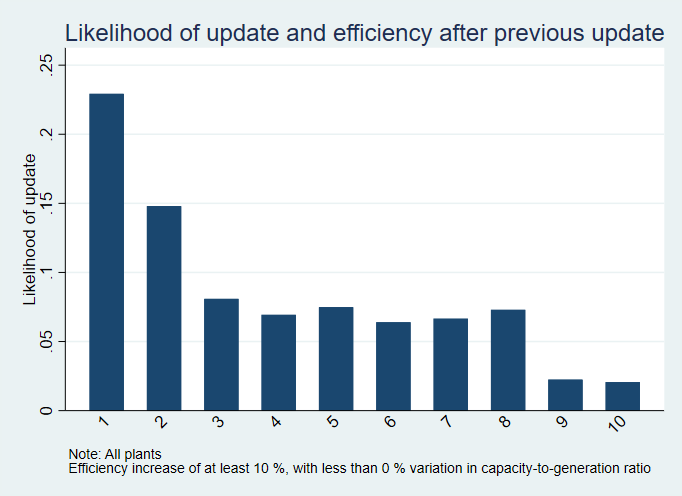
\includegraphics[scale=0.27]{hist_effic_updatedummy_all.png}
\end{figure}

\hyperlink{patterns_1gen}{\beamerbutton{Update pattern}}

\end{frame}
%%%%%%%%%%%%%%%%
\begin{frame}{Data: Adoption patterns}\label{updatespattern}

\begin{figure}
\caption{The likelihood of update and efficiency after previous update}
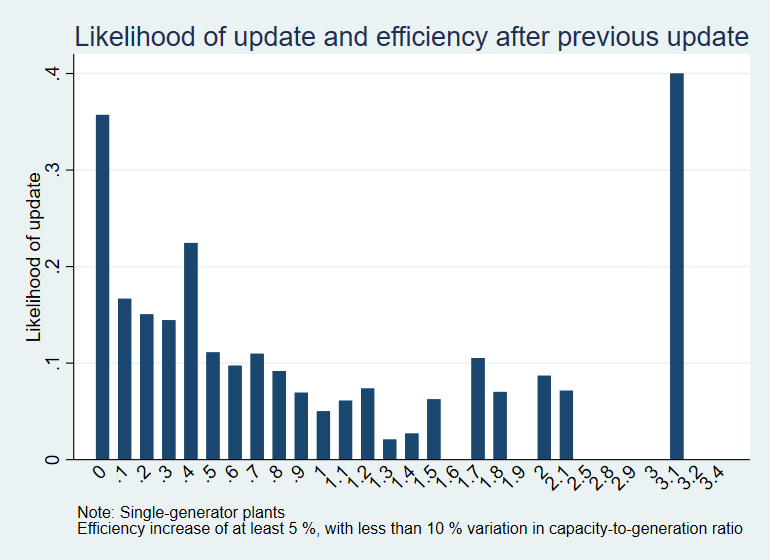
\includegraphics[scale=0.27]{hist_effic_updatedummy_1gen.png}
\end{figure}

\hyperlink{obscount}{\beamerbutton{Efficiency Distribution}}

\end{frame}
%%%%%%%%%%%%%%%%
\begin{frame}{Years since latest update}\label{Years since latest update}

\begin{figure}
\centering
\caption{Years since latest update, 2020}
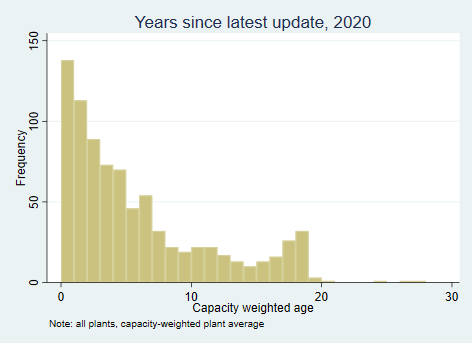
\includegraphics[scale=0.4]{hist_capage_2020_all.png}
\end{figure}
\scriptsize{Note: Technological update implies an efficiency increase of at least 10 \%, with less than 5 \% variation in generator capacity-to-generation ratio}

\hyperlink{efficall_dist}{\beamerbutton{All efficiency values}}
\hyperlink{variables}{\beamerbutton{Variables}}
\end{frame}
%%%%%%%%%%%%%%%
\begin{frame}{Calibration: efficiency in periods between updates}\label{effic_between_model}
\small
Firm decision:\\
\begin{align*} 
    v(a_{i},t) &= \max_{e_i,aot=\{0,1\}} p_E\frac{a_{i}^{1+\gamma t}}{(1+g_a)^t} e_i^\alpha -p_e e_i-c_f\\ 
    &+\beta \big(\mathbf{1}_{\{aot =0\}} \mathbb{E}[v(a_{i},t+1)] + \mathbf{1}_{\{aot =1\}}[ \mathbb{E}[v(a_{i}',t-\tau)]-c]\big)\\
\end{align*}
Between two updates the efficiency of a generator is then given by:\\
\begin{align*}
    a_{i,t} &= \frac{a_{i,t-s}}{(\frac{1+g_t}{a_{i,0}^\gamma})^s}  \rightarrow \ln a_{i,t} = \ln a_{i,t-s} -  s \ln(1+g_t) + s \gamma\ln a_{i,0} 
\end{align*}
where s is the number of years since the latest update.

    \hyperlink{gen_problem}{\beamerbutton{Model}}
    \hyperlink{transition1}{\beamerbutton{Transition 1}}
    \hyperlink{calibration}{\beamerbutton{Calibration table}}
\end{frame}

%%%%%%%%%%%%%%%

\begin{frame}{Regression results: efficiency in periods between updates}\label{effic_between_1gen}
\scriptsize
\begin{table}
\centering
\caption{Relative efficiency in periods between updates regressed on covariates}
\begin{tabular}{lcc} \hline
\scriptsize
 & (1) & (2) \\
VARIABLES & Raw data & Fixed effects \\ \hline
 &  &  \\
Years since latest update & -0.0140*** & -0.0316*** \\
 & (0.00338) & (0.00614) \\
Log relative efficiency after latest upgrade & 0.954*** & 0.459*** \\
 & (0.0157) & (0.0725) \\
Years since update, interaction with plant mean & 0.00239*** & 0.00277*** \\
 & (0.000368) & (0.000942) \\
Constant & -0.127*** & -0.0788*** \\
 & (0.00981) & (0.00997) \\
 &  &  \\
Observations & 3,092 & 2,964 \\
 Adjusted R-squared & 0.685 & 0.883 \\ \hline
\multicolumn{3}{c}{ Robust standard errors in parentheses} \\
\multicolumn{3}{c}{ *** p$<$0.01, ** p$<$0.05, * p$<$0.1} \\
\multicolumn{3}{c}{ Note: notes4} \\
\end{tabular}

\end{table}
\scriptsize{Note: Relative efficiency denotes efficiency relative to newly updated generators}

\hyperlink{effic_between_all}{\beamerbutton{All plants}}

\end{frame}

%%%%%%%%%%%%%%%%%%%%%%%%%%%
\begin{frame}{Efficiency in periods between updates, all plants}\label{effic_between_all}
\tiny
\begin{table}
\centering
\caption{Relative efficiency in periods between updates regressed on covariates}
\scriptsize
\begin{tabular}{lcc} \hline
 & (1) & (2) \\
VARIABLES & Raw data & Fixed effects \\ \hline
 &  &  \\
Capacity weighted age & -0.00458*** & -0.0146*** \\
 & (0.00145) & (0.00159) \\
Log relative efficiency after latest upgrade & 0.989*** & 0.400*** \\
 & (0.00807) & (0.0626) \\
Years since update, interaction with plant mean & 0.00110*** & 0.000740*** \\
 & (0.000144) & (0.000173) \\
Constant & -0.105*** & -0.00677 \\
 & (0.00433) & (0.00467) \\
 &  &  \\
Observations & 12,342 & 11,960 \\
 Adjusted R-squared & 0.695 & 0.850 \\ \hline
\multicolumn{3}{c}{ Robust standard errors in parentheses} \\
\multicolumn{3}{c}{ *** p$<$0.01, ** p$<$0.05, * p$<$0.1} \\
\multicolumn{3}{c}{ Note: notes4} \\
\end{tabular}

\end{table}
\scriptsize{Note: Relative efficiency denotes efficiency relative to newly updated generators}

\hyperlink{effic_between_1gen}{\beamerbutton{Single-generator plants}}

\end{frame}


%%%%%%%%%%%%%%%%

\begin{frame}{Power plant efficiency distribution, after update}\label{efficnew_dist}

\begin{figure}
\centering
\caption{Distribution of efficiency values after update, all plants}
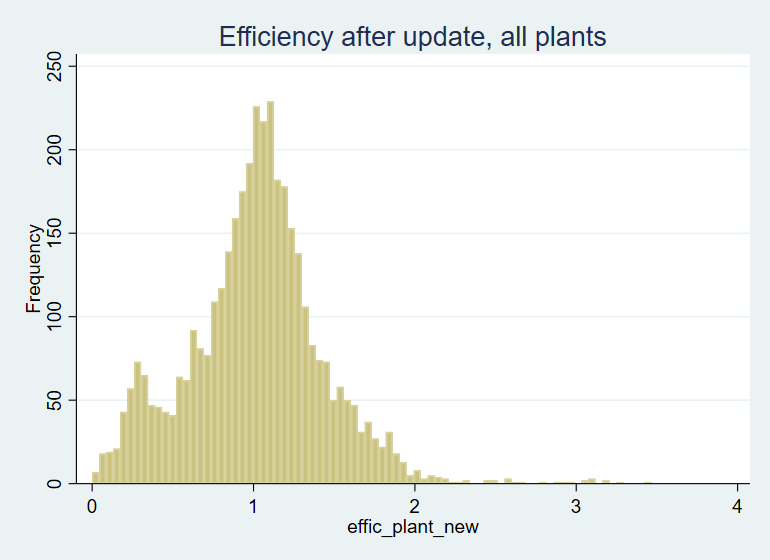
\includegraphics[scale=0.3]{EFFIC_all_efficnew_hist.png}
\end{figure}
\scriptsize{Note: Technological update implies an efficiency increase of at least 5 \%, with less than 10 \% variation in generator capacity-to-generation ratio}

\hyperlink{efficall_dist}{\beamerbutton{Efficiency Distribution}}
    
\end{frame}

%%%%%%%%%%%%%%%



\begin{frame}{Summary statistics, sample used in adoption regressions}
\input{summarystats_inpart4_10_5_all_sameN_small}
\footnotesize{Note: Adoption dummy defined as efficiency increase of at least 10\% with less than 5\% variation in the capacity-to-generation dummy }
    
\end{frame}
%%%%%%%%%%%%%%%




\end{document}


%%%%%%%%%%%%%%%
\begin{frame}{Patterns in the data: technology adoption}\label{Facts}

\begin{enumerate}
\item A generator's efficiency declines in the absence of technological updates.
\item A generator's efficiency is positively correlated with its efficiency after the latest update.
\item The likelihood of an update is positively correlated with the number of years since the latest update.
\item The likelihood of an update is negatively correlated with the generator's efficiency after the latest technological update. 
\item A generator's efficiency values after updates are highly correlated.
\end{enumerate}

\hyperlink{Data}{\beamerbutton{Data }}
    
\end{frame}
%%%%%%%%%%%%%%%
